%%%%%%%% ICML 2020 EXAMPLE LATEX SUBMISSION FILE %%%%%%%%%%%%%%%%%

\documentclass{article}

% Custom packages
\usepackage{amsthm}
\usepackage{amsmath}
\usepackage{amssymb}
\usepackage{blkarray}
\usepackage{mathtools}
\usepackage{multirow}
\usepackage{bm}
\usepackage{enumitem}
\usepackage{comment}
\def\sectionautorefname{Section}


%%%%%%%%%%%%%%%%%%%%%%%%%%%%
% Paper dependent stuff    %
%%%%%%%%%%%%%%%%%%%%%%%%%%%%

\newcommand{\Tau}{\mathcal{T}}

%%%%%%%%%%%%%%%%%%%%%%%%%%%%
% Aesthetics               %
% over-underline, hat, bold%
%%%%%%%%%%%%%%%%%%%%%%%%%%%%

\newcommand{\eps}{\varepsilon}
\newcommand{\vareps}{\varepsilon}
\renewcommand{\epsilon}{\varepsilon}
%\renewcommand{\hat}{\widehat}
\renewcommand{\tilde}{\widetilde}
\renewcommand{\bar}{\overline}

\newcommand*{\MyDef}{\mathrm{\tiny def}}
\newcommand*{\eqdefU}{\ensuremath{\mathop{\overset{\MyDef}{=}}}}% Unscaled version
% \newcommand*{\eqdef}{\mathop{\overset{\MyDef}{\resizebox{\widthof{\eqdefU}}{\heightof{=}}{=}}}}
\newcommand{\eqdef}{\stackrel{def}{=}}


\def\:#1{\protect \ifmmode {\mathbf{#1}} \else {\textbf{#1}} \fi}
\newcommand{\CommaBin}{\mathbin{\raisebox{0.5ex}{,}}}

\newcommand{\wt}[1]{\widetilde{#1}}
\newcommand{\wh}[1]{\widehat{#1}}
\newcommand{\wo}[1]{\overline{#1}}
\newcommand{\wb}[1]{\overline{#1}}

% bf and bm missing due to conflict!!
\newcommand{\bsym}[1]{\mathbf{#1}}
\newcommand{\bzero}{\mathbf{0}}
\newcommand{\ba}{\mathbf{a}}
\newcommand{\bb}{\mathbf{b}}
\newcommand{\bc}{\mathbf{c}}
\newcommand{\bd}{\mathbf{d}}
\newcommand{\be}{\mathbf{e}}
\newcommand{\bg}{\mathbf{g}}
\newcommand{\bh}{\mathbf{h}}
\newcommand{\bi}{\mathbf{i}}
\newcommand{\bj}{\mathbf{j}}
\newcommand{\bk}{\mathbf{k}}
\newcommand{\bl}{\mathbf{l}}
\newcommand{\bn}{\mathbf{n}}
\newcommand{\bo}{\mathbf{o}}
\newcommand{\bp}{\mathbf{p}}
\newcommand{\bq}{\mathbf{q}}
\newcommand{\br}{\mathbf{r}}
\newcommand{\bs}{\mathbf{s}}
\newcommand{\bt}{\mathbf{t}}
\newcommand{\bu}{\mathbf{u}}
\newcommand{\bv}{\mathbf{v}}
\newcommand{\bw}{\mathbf{w}}
\newcommand{\bx}{\mathbf{x}}
\newcommand{\by}{\mathbf{y}}
\newcommand{\bz}{\mathbf{z}}

\newcommand{\bA}{\mathbf{A}}
\newcommand{\bB}{\mathbf{B}}
\newcommand{\bC}{\mathbf{C}}
\newcommand{\bD}{\mathbf{D}}
\newcommand{\bE}{\mathbf{E}}
\newcommand{\bF}{\mathbf{F}}
\newcommand{\bG}{\mathbf{G}}
\newcommand{\bH}{\mathbf{H}}
\newcommand{\bI}{\mathbf{I}}
\newcommand{\bJ}{\mathbf{J}}
\newcommand{\bK}{\mathbf{K}}
\newcommand{\bL}{\mathbf{L}}
\newcommand{\bM}{\mathbf{M}}
\newcommand{\bN}{\mathbf{N}}
\newcommand{\bO}{\mathbf{O}}
\newcommand{\bP}{\mathbf{P}}
\newcommand{\bQ}{\mathbf{Q}}
\newcommand{\bR}{\mathbf{R}}
\newcommand{\bS}{\mathbf{S}}
\newcommand{\bT}{\mathbf{T}}
\newcommand{\bU}{\mathbf{U}}
\newcommand{\bV}{\mathbf{V}}
\newcommand{\bW}{\mathbf{W}}
\newcommand{\bX}{\mathbf{X}}
\newcommand{\bY}{\mathbf{Y}}
\newcommand{\bZ}{\mathbf{Z}}

% calligraphic
\newcommand{\cf}{\mathcal{f}}
\newcommand{\cA}{\mathcal{A}}
\newcommand{\cB}{\mathcal{B}}
\newcommand{\cC}{\mathcal{C}}
\newcommand{\cD}{\mathcal{D}}
\newcommand{\cE}{\mathcal{E}}
\newcommand{\cF}{\mathcal{F}}
\newcommand{\cG}{\mathcal{G}}
\newcommand{\cH}{\mathcal{H}}
\newcommand{\cI}{\mathcal{I}}
\newcommand{\cJ}{\mathcal{J}}
\newcommand{\cK}{\mathcal{K}}
\newcommand{\cL}{\mathcal{L}}
\newcommand{\cM}{\mathcal{M}}
\newcommand{\cN}{\mathcal{N}}
\newcommand{\cO}{\mathcal{O}}
\newcommand{\cP}{\mathcal{P}}
\newcommand{\cQ}{\mathcal{Q}}
\newcommand{\cR}{\mathcal{R}}
\newcommand{\cS}{\mathcal{S}}
\newcommand{\cT}{\mathcal{T}}
\newcommand{\cU}{\mathcal{U}}
\newcommand{\cV}{\mathcal{V}}
\newcommand{\cW}{\mathcal{W}}
\newcommand{\cX}{\mathcal{X}}
\newcommand{\cY}{\mathcal{Y}}
\newcommand{\cZ}{\mathcal{Z}}

%%%%%%%%%%%%%%%%%%%%%%%%%%%%
% Math jargon              %
%%%%%%%%%%%%%%%%%%%%%%%%%%%%
\newcommand{\wrt}{w.r.t.\xspace}
\newcommand{\defeq}{\stackrel{\mathclap{\normalfont\mbox{\tiny def}}}{=}}
\newcommand{\maxund}[1]{\max\limits_{#1}}
\newcommand{\supund}[1]{\text{sup}\limits_{#1}}
\newcommand{\minund}[1]{\min\limits_{#1}}
\renewcommand{\epsilon}{\varepsilon}
\newcommand{\bigotime}{\mathcal{O}}


\DeclareMathOperator*{\argmin}{arg\,min} 
\DeclareMathOperator*{\argmax}{arg\,max} 
\DeclareMathOperator*{\cupdot}{\mathbin{\mathaccent\cdot\cup}}

%%%%%%%%%%%%%%%%%%%%%%%%%%%%
% Matrix operators         %
%%%%%%%%%%%%%%%%%%%%%%%%%%%%
\newcommand{\transpose}{^\mathsf{\scriptscriptstyle T}}
\newcommand{\transp}{\mathsf{\scriptscriptstyle T}}
\DeclareMathOperator{\Tr}{Tr}
\DeclarePairedDelimiterX{\inp}[2]{\langle}{\rangle}{#1, #2}

%%%%%%%%%%%%%%%%%%%%%%%%%%%%
% Statistic operators      %
%%%%%%%%%%%%%%%%%%%%%%%%%%%%
\newcommand{\probability}[1]{\mathbb{P}\left(#1\right)}
\newcommand{\probdist}{Pr}
\DeclareMathOperator*{\expectedvalue}{\mathbb{E}}
\DeclareMathOperator*{\variance}{\text{Var}}
\newcommand{\expectedvalueover}[1]{\expectedvalue\limits_{#1}}
\newcommand{\condbar}{\;\middle|\;}
\newcommand{\gaussdistr}{\mathcal{N}}
\newcommand{\uniformdistr}{\mathcal{U}}
\newcommand{\bernoullidist}{\mathcal{B}}

%%%%%%%%%%%%%%%%%%%%%%%%%%%%
% Algebraic Sets           %
%%%%%%%%%%%%%%%%%%%%%%%%%%%%
\newcommand{\Real}{\mathbb{R}}
\newcommand{\Natural}{\mathbb{N}}
\newcommand{\statespace}{\mathcal{X}}
\newcommand{\funcspace}{\mathcal{F}}
\newcommand{\dynaspace}{\mathcal{T}}


\newtheorem{theorem}{Theorem}
\newtheorem{definition}{Definition}
\newtheorem{lemma}{Lemma}
\newtheorem{proposition}{Proposition}
\providecommand*\propositionautorefname{Proposition}
\newtheorem{remark}{Remark}
\newtheorem{property}{Property}
\newtheorem{assumption}{Assumption}
\providecommand*\assumptionautorefname{Assumption}
\newtheorem{conjecture}{Conjecture}

\newtheorem*{definition*}{Definition}
\newtheorem*{theorem*}{Theorem}
\newtheorem*{proposition*}{Proposition}
\newtheorem*{remark*}{Remark}
\newtheorem*{example*}{Example}

% Recommended, but optional, packages for figures and better typesetting:
\usepackage{microtype}
\usepackage{graphicx}
\usepackage{subfigure}
\usepackage{booktabs} % for professional tables

% hyperref makes hyperlinks in the resulting PDF.
% If your build breaks (sometimes temporarily if a hyperlink spans a page)
% please comment out the following usepackage line and replace
% \usepackage{icml2020} with \usepackage[nohyperref]{icml2020} above.
\usepackage{hyperref}

% Attempt to make hyperref and algorithmic work together better:
\newcommand{\theHalgorithm}{\arabic{algorithm}}

% Use the following line for the initial blind version submitted for review:
\usepackage{icml2020}

% If accepted, instead use the following line for the camera-ready submission:
%\usepackage[accepted]{icml2020}

% The \icmltitle you define below is probably too long as a header.
% Therefore, a short form for the running title is supplied here:
\icmltitlerunning{Robust Estimation, Prediction and Control}

\begin{document}
	
	\twocolumn[
	\icmltitle{Robust Estimation, Prediction and Control with \\ Linear Dynamics and Generic Costs}
	
	% It is OKAY to include author information, even for blind
	% submissions: the style file will automatically remove it for you
	% unless you've provided the [accepted] option to the icml2020
	% package.
	
	% List of affiliations: The first argument should be a (short)
	% identifier you will use later to specify author affiliations
	% Academic affiliations should list Department, University, City, Region, Country
	% Industry affiliations should list Company, City, Region, Country
	
	% You can specify symbols, otherwise they are numbered in order.
	% Ideally, you should not use this facility. Affiliations will be numbered
	% in order of appearance and this is the preferred way.
	\icmlsetsymbol{equal}{*}
	
	\begin{icmlauthorlist}
		\icmlauthor{Edouard Leurent}{seq,val,ren}
		\icmlauthor{Denis Efimov}{val}
		\icmlauthor{Odalric Ambrym-Maillard}{seq}
	\end{icmlauthorlist}
	
	\icmlaffiliation{seq}{Inria Lille Nord-Europe, Sequel Project, Lille, France}
	\icmlaffiliation{val}{Inria Lille Nord-Europe, Valse Project, Lille, France}
	\icmlaffiliation{ren}{Renault Group, Guyancourt, France}
	
	\icmlcorrespondingauthor{Edouard Leurent}{edouard.leurent@inria.fr}
	
	% You may provide any keywords that you
	% find helpful for describing your paper; these are used to populate
	% the "keywords" metadata in the PDF but will not be shown in the document
	\icmlkeywords{Machine Learning, ICML}
	
	\vskip 0.3in
	]
	
	% this must go after the closing bracket ] following \twocolumn[ ...
	
	% This command actually creates the footnote in the first column
	% listing the affiliations and the copyright notice.
	% The command takes one argument, which is text to display at the start of the footnote.
	% The \icmlEqualContribution command is standard text for equal contribution.
	% Remove it (just {}) if you do not need this facility.
	
	\printAffiliationsAndNotice{}  % leave blank if no need to mention equal contribution
%	\printAffiliationsAndNotice{\icmlEqualContribution} % otherwise use the standard text.
	
\begin{abstract}
We develop a framework for the adaptive model predictive control of a linear system with unknown parameters and arbitrary bounded costs, in a critical setting where failures are costly and should be prevented at all time.  Our approach builds on two ideas: first, we incorporate prior knowledge of the dynamics in the form of a known structure that shapes uncertainty, which can be tightened as we collect interaction data by building high-confidence regions through least-square regression. Second, in order to handle this uncertainty we formulate a robust control objective. Leveraging tools from the interval prediction literature, we convert the confidence regions on parameters into confidence sets on trajectories induced by the controls. These controls are then optimised resorting to tree-based planning methods. We eventually relax our modeling assumptions with a multi-model extension based on a data-driven robust model selection mechanism. The full procedure is designed to produce reasonable and safe behaviours at deployment while recovering an asymptotic optimality. We illustrate it on a practical case of autonomous driving at a crossroads intersection among vehicles with uncertain behaviours.\footnote[2]{Source code and videos are available in the Supplementary Material}
\end{abstract}	

\section{Introduction}

Despite the recent successes of Reinforcement Learning in cracking many hard problems \citep[e.g.][]{mnih2015humanlevel,Silver1140}, this tool has hardly been applied in real industrial issues. This could be attributed to two undesirable properties which limit its practical applications. First, it depends on a tremendous amount of interaction data that cannot always be simulated. This issue is alleviated by model-based methods -- which we consider in this work -- that benefit from better sample efficiencies by exploiting a richer data stream than their model-free counterparts. Second, it relies on trial-and-error and random exploration. In this paper, we consider the problem of controlling an unknown linear system $x(t)$ so as to maximise an \emph{arbitrary} bounded reward function $R$, in a critical setting where mistakes are costly and must be avoided at all time. 
This choice of rich reward space is crucial to have sufficient flexibility to model non-convex and non-smooth functions that naturally arise in many practical problems involving combinatorial optimisation, branching decisions, etc., while quadratic costs are mostly suited for tracking a reference trajectory already known a priori \citep[e.g.][]{Kumar2013}.

Since experiencing failures is out of question, the only way to prevent them from the outset, when the system is first deployed, is to rely on some sort of prior knowledge. In this work, we assume that the system dynamics are partially known, in the form of a parametrized dynamical system with unknown parameters. We argue that this assumption is realistic given that most industrial applications to date have been relying on physical models to describe their processes and well-engineered controllers to operate them, rather than machine learning. Our framework relaxes this modelling effort by allowing some \emph{structured uncertainty} around the nominal model. We adopt a data-driven scheme where we wish to estimate the parameters more accurately as we interact with the true system. Most model-based reinforcement learning algorithms rely on the estimated dynamics to derive the corresponding optimal controls \citep[e.g.][]{Lenz2015,Levine2015}, but suffer from \emph{model bias}: they ignore the error that exists between the learned and true dynamics, which can dramatically degrade the control performances \citep{Schneider1997}. It is particularly likely when maximising an objective under constraints, which naturally pushes the systems to operate in the vicinity of constraint saturation and makes it prone to failure.

To address this issue, we turn to the framework of \emph{robust} decision-making \citep{Bental2009,Bertsimas2011,Gorissen2015}: instead of merely considering a point estimate of the dynamics, we build an entire \emph{confidence region} that contains the true dynamics with high probability, and optimise the decisions so as to maximise the worst-case outcome with respect to this uncertainty. Maximin problems are notoriously hard to solve, and all the more in our setting where the reward function $R$ is generic. In particular, this excludes a number of tools from the robust synthesis literature, such as $\cH_\infty$ control \citep[see, e.g.][]{Basar1996} or system-level synthesis \citep{Dean2017,Dean2018}. We turn instead to more general planning algorithms. The continuous state space prevents us from using dynamic programming techniques, so we consider tree-based planning instead. Though there exist works addressing continuous actions \citep{Busoniu2018,Weinstein2012}, we resort to a first approximation and discretise the decision space by adopting a hierarchical control architecture. At each time, the agent can select low-level controller to execute among a finite basis, e.g. choose a short-term goal to reach or a skill to execute such as a driving maneuver. The discretisation induces a suboptimality, but it can be mitigated by diversifying the controller basis. Tree-based planning algorithms are relevant in this context of discrete actions, but are only designed for a single known generative model instead of an entire confidence region for the system dynamics. We adapt them to the robust framework by following a two-steps procedure: we first predict a set of states that can be reached under a planned control sequence with respect to all possible dynamics. This reachability set is used to provide a conservative pessimistic reward to the planning algorithm. The next section aims to clarify and formalize these ideas, and state our contributions.


\subsection{Problem Statement and Our Contributions}

\paragraph{Notation}

The dynamics of the real system are described in continuous time. However, all the sensing and control performed on-board happen in discrete time, with time-step $\dd t>0$. For any variable $z$, we use the subscript notation to refer to these discrete times: $z_n = z(t_n)$ with $t_n = n\dd t$ and $n\in\Natural$. We use bold symbols to denote temporal sequences $\bz = (z_n)_{n\in\Natural}$. We denote $z^+ = \max(z,0)$, $z^- = z^+-z$, $|z| = z^++z^-$ and $[n]=\{1,2,\dots, n\}$.

\paragraph{Structured dynamics}
We consider a linear system with state $x\in\Real^p$, acted on by controls $u\in\Real^q$ and perturbations $\omega\in\Real^r$, and following dynamics in the form:
\begin{equation}
\label{eq:dynamics}
\dot{x}(t)=A(\theta)x(t) + B u(t) + D \omega(t),\;t\geq0.
\end{equation}
 It is assumed that the parameter vector $\theta$ in the state matrix $A(\theta)\in\Real^{p\times p}$ belongs to a compact set $\Theta \subset \Real^d$. The control matrix $B\in\Real^{p\times q}$ and disturbance matrix $D\in\Real^{p\times r}$ are known. We also assume having access to the observation of $x(t)$ and to a noisy measurement of $\dot{x}(t)$ in the form $y(t)=\dot{x}(t) + C\nu(t)$, where $\nu(t)\in\Real^s$ is a measurement noise and $C\in\Real^{p\times s}$ is known. Assumptions over the disturbance $\omega$ and noise $\nu$ will be detailed further, and we denote $\eta(t) = C\nu(t) + D\omega(t)$. 
 
 Our goal is to design a robust model predictive control for \eqref{eq:dynamics}, and to this end the following steps will be performed and explained later in details.

\paragraph{Model estimation}


\begin{figure}[t]
	\centering
	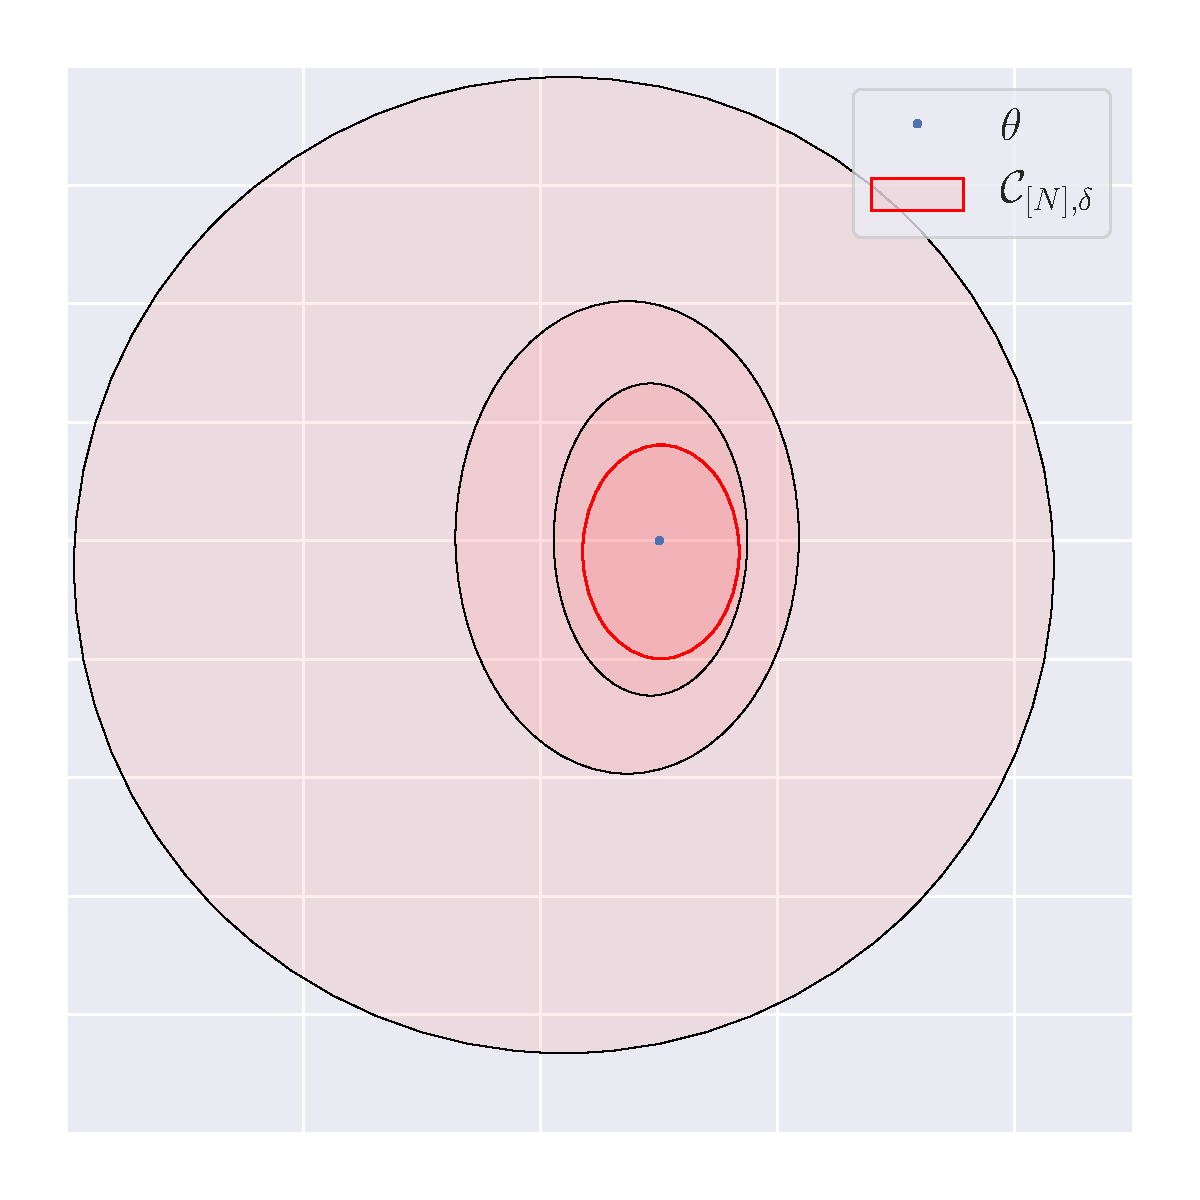
\includegraphics[trim={0 2cm 0 0}, clip, width=0.6\linewidth]{img/ellipsoid}
	\caption{The model estimation procedure, running on the obstacle avoidance problem of \autoref{sec:experiments}. The confidence region $C_{[N],\delta}$ shrinks with the number of samples $N$.}
	\label{fig:estimation}
\end{figure}

\begin{figure}[t]
	\centering
	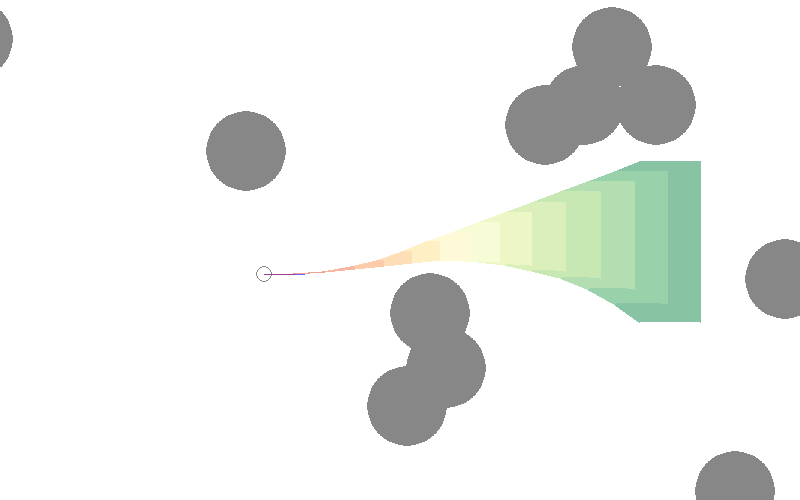
\includegraphics[width=0.8\linewidth]{img/obstacle_small}
	\caption{The state prediction procedure running on the obstacle avoidance problem of \autoref{sec:experiments}. At each time step (red to green), we bound the set of reachable states under model uncertainty \eqref{eq:confidence}}
	\label{fig:prediction}
\end{figure}

In \autoref{sec:estimation}, having observed history of transitions $\cD_{[N]} = \{(x_n, y_n,u_n)\}_{n\in[N]}$, and given a confidence level $\delta\in(0, 1)$, we wish to find a confidence region $\cC_{[N],\delta} \subset \Theta$ as tight as possible and such that it holds:
\begin{align}
\probability{A(\theta)\in \cC_{[N],\delta}} \geq 1-\delta
\label{eq:confidence}
\end{align}
Such regions are illustrated in \autoref{fig:estimation}. Our first contribution extends the work of \citet{Abbasi2011} who provide a confidence ellipsoid for the regularised least-square estimator to our setting of feature matrices, rather than feature vectors.

\paragraph{Robust objective}

At the time step $n=N$, considering the confidence region $\cC_{[N],\delta}$ obtained in the model estimation phase, we formulate our robust control objective:
\begin{equation}
\label{eq:robust-control}
\sup_{\bu\in{(\Real^q)}^\Natural} \underbrace{\inf_{\substack{A(\theta) \in \cC_{[N],\delta} \\ \bom\in[\underline{\bom},\overline{\bom}]^\Natural}} \left[\sum_{n=N+1}^\infty \gamma^n R(x_n(\bu,\bom))\right]}_{V^r(\bu)}
\end{equation}
where $\gamma\in(0,1)$ is a discount factor. The rest of the paper tackles the optimisation of \eqref{eq:robust-control}.

\paragraph{State prediction}

Maximin problems such as \eqref{eq:robust-control} are notoriously difficult to solve even in cases such where the reward $R$ has a simple form. With arbitrary functions $R$, we cannot hope to derive a solution in explicit form. Our second contribution is to propose to solve \eqref{eq:robust-control} numerically by adopting a \emph{predict-then-optimise} scheme. In \autoref{sec:prediction}, we aim to derive a \emph{set predictor} $X(t)$ for the system \eqref{eq:dynamics}, illustrated in \autoref{fig:prediction}. This predictor takes the information on the observed current state ${x}_N$, a confidence region $\cC_\delta$ verifying \eqref{eq:confidence}, a planned control sequence $\bu$ and some admissible bounds on the perturbation $[\underline{\omega}(t),\overline{\omega}(t)]$; and outputs a set $X(t)$ that must verify the \emph{inclusion property}:
\begin{equation}
\label{eq:inclusion-generic}
 x(t)\in X(t),\quad\forall t\geq t_N.
\end{equation}
We leverage recent results from the uncertain system simulation literature to efficiently compute such a predictor.

\paragraph{Robust planning}

Since $R$ is generic, potentially non-smooth and non-convex, solving the optimal -- not to mention the robust -- control objective in the original continuous control space $(\Real^q)^\Natural$ is intractable.
In this work, we choose to approximate the solution of \eqref{eq:robust-control} by optimising over a finite set of \emph{actions} $\cA$. Each action $a\in\cA$ corresponds to the selection of a low-level controller $\pi_a$, that we take affine:
\[u(t) = \pi_a(x(t)) \eqdef -K_a x(t) + u_a.\]
For instance, a tracking a subgoal $x_g$ can be achieved with $\pi_g = K(x_g - x)$. The robust objective \eqref{eq:robust-control} becomes 
\begin{equation}
\label{eq:robust-control-disc}
\sup_{\ba\in{\cA}^\Natural} \underbrace{\inf_{\substack{A(\theta) \in \cC_{[N],\delta} \\ \bom\in[\underline{\bom},\overline{\bom}]^\Natural}} \left[\sum_{n=N+1}^\infty \gamma^n R(x_n(\ba,\bom))\right]}_{V^r(\ba)},
\end{equation}
where $x_n(\ba, \bom)$ stems from \eqref{eq:dynamics} with $u_n = \pi_{a_n}(x_n)$.

In \autoref{sec:control}, facing a sequential decision problem with continuous states and discrete actions, we turn to the literature of tree-based planning algorithms. Our third contribution adapts them to the robust objective \eqref{eq:robust-control-disc} by approximating it with a tractable surrogate $\hat{V}^r$ that exploits the set predictor \eqref{eq:inclusion-generic} to define a pessimistic reward. In our main result, we show that the best surrogate performance achieved during planning is guaranteed to be attained on the true system, and provide an upper bound for the approximation gap and simple regret of our framework in \autoref{thm:control-error}.

The \autoref{alg:full} shows the full integration of the three procedures of estimation, prediction and control. 

\paragraph{Model selection} In \autoref{sec:multi-model}, our forth contribution extends the proposed framework to consider multiple modelling assumptions, while narrowing uncertainty through data-driven model rejection, and still ensuring safety via robust model-selection during planning.

\paragraph{Experiments} Finally, in \autoref{sec:experiments} we demonstrate the applicability of our proposed \autoref{alg:full} in two numerical experiments. First, a simple illustrative example and then, a more challenging simulation for safe autonomous driving.

\begin{algorithm}[tb]
	\caption{Robust Estimation, Prediction and Control}
	\label{alg:full}
	\begin{algorithmic}
		\STATE {\bfseries Input:} confidence level $\delta$, structure $(A,\phi)$, reward $R$
		\STATE $\cD_{[0]}\gets\emptyset,\, \ba_1\gets\emptyset$
		\FOR{$N = 0,1,2,\dots$} 
		\STATE $\cC_{[N],\delta} \gets$\textsc{Model Estimation}$(\cD_{[N]})$. \eqref{eq:polytope}
		\FOR{each planning step $k\in[K]$}
		\FOR{each action $b\in \cA$}
		\STATE $[\underline{x}_{n+1}, \overline{x}_{n+1}]\gets$ \textsc{Interval Prediction}(
		\STATE $\qquad\qquad\qquad\qquad\cC_{[N],\delta}, \ba_kb$). \eqref{eq:interval-predictor}
		\ENDFOR
		\STATE $\ba_{k+1}$ $\gets$\textsc{Pessimistic Planning}$($
		\STATE$\qquad\qquad\underline{R_{n+1}}([\underline{x}_{n+1}, \overline{x}_{n+1}]))$.  \eqref{eq:opd}
		\ENDFOR
		\STATE Execute the recommended control $u_{N+1}$, and add the observed transition $(x_{N+1}, y_{N+1}, u_{N+1})$ to $\cD_{[N+1]}$.
		\ENDFOR
	\end{algorithmic}
\end{algorithm}

\subsection{Related Work}

\paragraph{Linear-quadratic problems} There is a rich body of literature dedicated to the study of linear systems with quadratic costs, and we focus on those providing non-asymptotic results when the system parameters $A, B$ are unknown. In their seminal work \citet{abbasi-yadkori11a}, consider the problem of cumulative regret minimisation. They follow the \emph{Optimism in the Face of Uncertainty} paradigm from the multi-armed bandit literature, that consists in selecting the best possible dynamics within a high-confidence region while enforcing a controllability constraint, and computing the corresponding optimal control in closed-form by solving a Riccati equation. They show that this procedures achieves a $\tilde{\cO}\left(N^{1/2}\right)$ cumulative regret. \citep{Ibrahimi2013,Faradonbeh2017} adapt these results to the case of sparse dynamics. \citet{Ouyang2017,abeille18a} provide the same result by applying Thomson Sampling rather of optimism to select a dynamical model, and rejection sampling to enforce the controllability constraint. These methods aim at regret minimization to quickly reduce uncertainty, through information-seeking behaviours. Other works use noise injection for exploration such as \citep{Dean2017,Dean2018}. However, neither optimism and cumulative regret minimization nor random exploration fit a critical setting, where ensuring safety as a top priority requires instead to consider the pessimistic outcomes.
The work of \citet{Dean2017} is closest to our setting: after an offline estimation phase, where the controls do not aim at regret minimization, they estimate a simple regret between a robust controller and the optimal performance. Our work mainly differs in that it addresses generic costs and forbids random exploration.

\paragraph{Robust planning}
Robust optimization with generic costs has also been studied in the context of finite Markov Decision Processes with uncertain parameters by \citet{Iyengar2005}, \citet{Nilim2005} and \citet{Wiesemann2013}. They showed that the main results of Dynamic Programming can be extended to their robust counterparts only when the dynamics ambiguity set verifies a certain rectangularity property, that amounts to an independence assumption between the uncertainty sets of each transition and is related to time-varying uncertainty. Since our setting requires dealing with continuous states and time-invariant uncertainty, these methods do not apply.

\section{Model Estimation}

\label{sec:estimation}

To derive a confidence region for the dynamical parameters $\theta$, the functional relationship $A(\theta)$ must be specified.
\begin{assumption}[Structure]
\label{assumpt:structure}
There exists a known feature tensor $\phi\in \Real^{d \times p \times p}$ such that for all $\theta\in\Theta$,
\begin{equation}
    A(\theta) = A + %\theta^\transp \phi \eqdef A + 
    \sum_{i=1}^d \theta_i\phi_i,
\end{equation}
where $A,\phi_1,\dots,\phi_d\in\Real^{p\times p}$ are known. For all $n$, we denote $\Phi_n = [\phi_1 x_n \dots \phi_d x_n]\in\Real^{p\times d}$.

We also assume to know a bound $S$ such that $\theta\in[-S,S]^d$.
\end{assumption}

We abuse notations and define a virtual measurement signal, still denoted $y(t)$, that includes additional known terms
\begin{equation*}
%\label{eq:measurement}
    y(t) = \dot{x}(t) + C\nu(t) - A x(t) - Bu(t),
\end{equation*}
to obtain a linear regression system
$
y_n = \Phi_n\theta + \eta_n.
$

\paragraph{Regularised least square} To derive an estimate on $\theta$, we consider the weighted $L_2$-regularised regression problem with weights  $\Sigma_p\in\Real^{p\times p}$ and parameter $\lambda\in\Real^+_*$:
\begin{equation}
    \label{eq:regression_min}
    \min_{\theta\in\Real^d} \sum_{n=1}^N \|y_n -\Phi_n\theta\|_{\Sigma_p^{-1}}^2 + \lambda\|\theta\|_{}^2.
\end{equation}


The solution can be obtained as:

\begin{proposition}[Regularised solution]
\label{prop:regularized_solution}
The solution to \eqref{eq:regression_min} is
\begin{align}
    \label{eq:vector_rls}
    \theta_{N,\lambda} &= G_{N, \lambda}^{-1} \sum_{n=1}^N \Phi_n^\transp \Sigma_p^{-1} y_n,\\
	\label{eq:g_n_lambda}
    \text{where }\quad G_{N, \lambda} &= \sum_{n=1}^N \Phi_{n}^\transp\Sigma_p^{-1}\Phi_{n}  + \lambda I_d \in \Real^{d\times d}.
\end{align}
\end{proposition}

Substituting $y_n$ into \eqref{eq:vector_rls} yields the regression error:
\begin{align}
    \theta_{N,\lambda} - \theta = G_{N, \lambda}^{-1}\sum_{n=1}^N \Phi_n^\transp \Sigma_p^{-1}\eta_n - \lambda G_{N, \lambda}^{-1}\theta.
\end{align}


Depending on the assumption we have over the noise $\eta_n$, we can bound this error in different ways.


\subsection{Bounded noise}

\begin{assumption}[Bounded noise]
\label{assumpt:bounded-noise}
The noise $\eta(t)$ is bounded in $\|\cdot\|_\infty$.
\end{assumption}

In particular, we denote the coefficient-wise bounds over perturbations as $\underline{\omega}(t) \leq \omega(t) \leq \overline{\omega}(t)$. This is a deterministic assumption, then by Hölder inequality a confidence region $\cC_{[N],0}$ can be derived based on a $L_1$-ball estimate of $\theta$ at time $N$, i.e. a polytope with $2d$ vertices:
\begin{equation}
\label{eq:bounded-noise-polytope}
\|\theta_{N,\lambda}\! -\! \theta\|_1\! \leq \! \|G_{N, \lambda}^{-1}\!\sum_{n=1}^N \!\Phi_n^\transp\! \Sigma_p^{-1}\!\|_1\|\eta\|_\infty\! +\!\lambda\|G_{N, \lambda}^{-1}\!\|_1S
\end{equation}

There may be cases where \autoref{assumpt:bounded-noise} does not hold. For instance, when the noise $\eta$ is Gaussian, then $\|\eta\|_\infty=+\infty$ which makes \eqref{eq:bounded-noise-polytope} uninformative. Then, another probabilistic assumption can be made.

\subsection{Sub-Gaussian noise}

\begin{assumption}[Sub-Gaussian Noise]
\label{assumpt:gaussian-noise}
At each time $t\geq0$ the noise $\eta(t)$ is an independent sub-Gaussian noise with covariance proxy $\Sigma_p \in \Real^{p\times p}$:
\begin{equation*}
    \forall u\in\Real^p,\, \expectedvalue \left[ \exp{\left( u^\transp \eta(t)\right)}\right] \leq \exp{\left( \frac{1}{2} u^\transp \Sigma_p u\right)}.
\end{equation*}
\end{assumption}
For instance, it is the case when $\nu$ and $\omega$ are Gaussian noises with covariance matrices $\Sigma_r$ and $\Sigma_s$, with $\Sigma_p \eqdef C\Sigma_r C^\transp + D\Sigma_s D^\transp$. Note that \autoref{assumpt:bounded-noise} implies that $\eta$ is sub-Gaussian with covariance proxy $\Sigma_p=\|\eta\|_\infty I_p$.

\begin{theorem}[Confidence ellipsoid, a matricial version of \citealt{Abbasi2011}]
\label{thm:confidence_ellipsoid}
Under \autoref{assumpt:gaussian-noise}, it holds with probability at least $1-\delta$ that
\begin{align}
    \label{eq:confidence-ellipsoid}
    \| \theta_{N,\lambda}  - \theta\|_{G_{N,\lambda}} \leq \beta_N(\delta),
\end{align}
with
\begin{equation}
	\label{eq:beta_n}
    \beta_N(\delta)\eqdef \sqrt{2\ln \left(\frac{\det(G_{N,\lambda})^{1/2}}{\delta\det(\lambda I_d)^{1/2}}\right)}
     + (\lambda d)^{1/2}S.
\end{equation}
\end{theorem}

We can enclose this confidence ellipsoid $\eqref{eq:confidence-ellipsoid}$ into a polytope $C_{[N],\delta}$. For simplicity, we present here a simple but coarse strategy: bound the ellipsoid by its enclosing sphere, and then the sphere by its enclosing hypercube. We obtain
\begin{align}
    \label{eq:polytope}
     &\cC_{[N],\delta} = \left\{ A_{0}+\sum_{i=1}^{2^d}\alpha_{i}\Delta A_{i}: \alpha\geq 0,  \sum_{i=1}^{2^d}\alpha_{i}=1\right\}
\end{align}
where $A_{0,N} = A + \theta_{N,\lambda}^\transp\phi, \Delta A_{i} = {h_i} \sqrt{\frac{\beta_N(\delta)}{\lambda_{\max}(G_{N,\lambda})}}, h_i\in\{-1,1\}^d$. Another strategy presented in the Supplementary Material produces a much tighter polytope, at the price of an increased computational cost required by the diagonalisation of $G_{N,\lambda}$.

\paragraph{Remark} The robust objective \eqref{eq:robust-control} involves bounds $\underline{\omega}(t)\leq \omega(t) \leq \overline{\omega}(t)$ over the possible perturbations we want to protect against. In the unbounded sub-Gaussian noise setting of \autoref{assumpt:gaussian-noise}, we can use the same formulation by deriving local high-confidence bounds that each holds with confidence $\delta_n$. By choosing $\delta_n = \frac{\delta}{n(n+1)}$, the event $\{\forall n, \underline{\omega}(t_n) \leq \omega(t_n) \leq \overline{\omega}(t_n)\}$ holds with probability $1-\delta$.

\section{State Prediction}

\label{sec:prediction}

To study the inclusion property \eqref{eq:inclusion-generic}, we must start by choosing a set representation $X(t)$. We consider interval prediction, rather than zonotope prediction for instance \citep[e.g.][]{le2012}, for the sake of simplicity of implementation and computational efficiency. We represent an interval as $X(t) = [\underline{x}(t), \overline{x}(t)]\in \Real^p\times \Real^p$, and \eqref{eq:inclusion-generic} becomes:
\begin{equation}
\label{eq:inclusion-property}
\underline{x}(t)\leq x(t)\leq\overline{x}(t),\quad\forall t\geq t_N.
\end{equation} 

A simple solution to \eqref{eq:inclusion-property} is proposed in \citep{Efimov2012}, where, given bounds $\underline{A}\leq A(\theta)\leq\overline{A}$ from $\cC_{[N],\delta}$ they use matrix interval arithmetic to derive the predictor:
\begin{proposition}[Simple predictor of \citealt{Efimov2012}]
Assuming that \eqref{eq:confidence} is satisfied for the system \eqref{eq:dynamics}, then the interval predictor:
\begin{eqnarray}
\dot{\underline{x}}(t) & = & \underline{A}^{+}\underline{x}^{+}(t)-\overline{A}^{+}\underline{x}^{-}(t)-\underline{A}^{-}\overline{x}^{+}(t) +\overline{A}^{-}\overline{x}^{-}(t)\nonumber \\
 &  &+Bu(t) + D^{+}\underline{\omega}(t)-D^{-}\overline{\omega}(t),\label{eq:predictor-naive}\\
\dot{\overline{x}}(t) & = & \overline{A}^{+}\overline{x}^{+}(t)-\underline{A}^{+}\overline{x}^{-}(t)-\overline{A}^{-}\underline{x}^{+}(t)+\underline{A}^{-}\underline{x}^{-}(t)\nonumber \\
 &  &+Bu(t) + D^{+}\overline{\omega}(t)-D^{-}\underline{\omega}(t),\nonumber \\
 &  & \underline{x}(t_N)=\overline{x}(t_N)={x}(t_N),\nonumber 
\end{eqnarray}
ensures the inclusion property \eqref{eq:inclusion-property} with confidence level $\delta$.
\end{proposition}

However, \citet{leurent2019interval} showed that this predictor can have unstable dynamics, even for stable systems, which causes a fast build-up of uncertainty. They proposed an enhanced predictor which exploits the polytopic structure \eqref{eq:polytope} to produce tighter and more stable predictions, at the price of an additional requirement:

\begin{assumption}
\label{assumpt:metzler}
There exists an orthogonal matrix $Z\in\Real^{p\times p}$ such that $Z^\transp A_0 Z$ is Metzler\footnote{We say that a matrix is Metlzer when all its non-diagonal coefficients are non-negative.}.
\end{assumption}
In practice, this assumption is often verified. It is for instance the case whenever $A_0$ is diagonalisable. The similarity transformation of \citep{Efimov2013} provides a method to compute such $Z$ when the system is observable. To simplify the notation, we will further assume that $Z = I_p$. Denote $
\Delta A_{+}=\sum_{i=1}^{2^d}\Delta A_{i}^{+},\;\Delta A_{-}=\sum_{i=1}^{2^d}\Delta A_{i}^{-}$.
% The similarity transformation of \citep{Efimov_a2013} provides a method to compute such $P$ whenever there exist $C_1,C_2$ which make $(A(\theta), C_1)$ and $(A_0, C_2)$ observable.
% Under this assumption, without loss of generality up to a change of basis $x\rightarrow P^{-1}x$ that we do not write for the sake of readability, this assumption is equivalent to considering that $A_0$ itself is Metzler.

\begin{proposition}[Enhanced predictor of \citealt{leurent2019interval}]
\label{prop:predictor}
Assuming that \eqref{eq:polytope} and \autoref{assumpt:metzler} are satisfied for the system \eqref{eq:dynamics}, then the interval predictor:
\begin{eqnarray}
\dot{\underline{x}}(t) & = & A_{0}\underline{x}(t)-\Delta A_{+}\underline{x}^{-}(t)-\Delta A_{-}\overline{x}^{+}(t)\nonumber \\
 &  & +Bu(t)+D^{+}\underline{\omega}(t)-D^{-}\overline{\omega}(t),\nonumber\\
\dot{\overline{x}}(t) & = & A_{0}\overline{x}(t)+\Delta A_{+}\overline{x}^{+}(t)+\Delta A_{-}\underline{x}^{-}(t) \label{eq:interval-predictor} \\
 &  & +Bu(t)+D^{+}\overline{\omega}(t)-D^{-}\underline{\omega}(t),\nonumber \\
 &  & \underline{x}(t_N)=\overline{x}(t_N)={x}(t_N)\nonumber 
\end{eqnarray}
ensures the inclusion property \eqref{eq:inclusion-property} with confidence level $\delta$..
\end{proposition}

\begin{figure}[tp]
	\centering
	{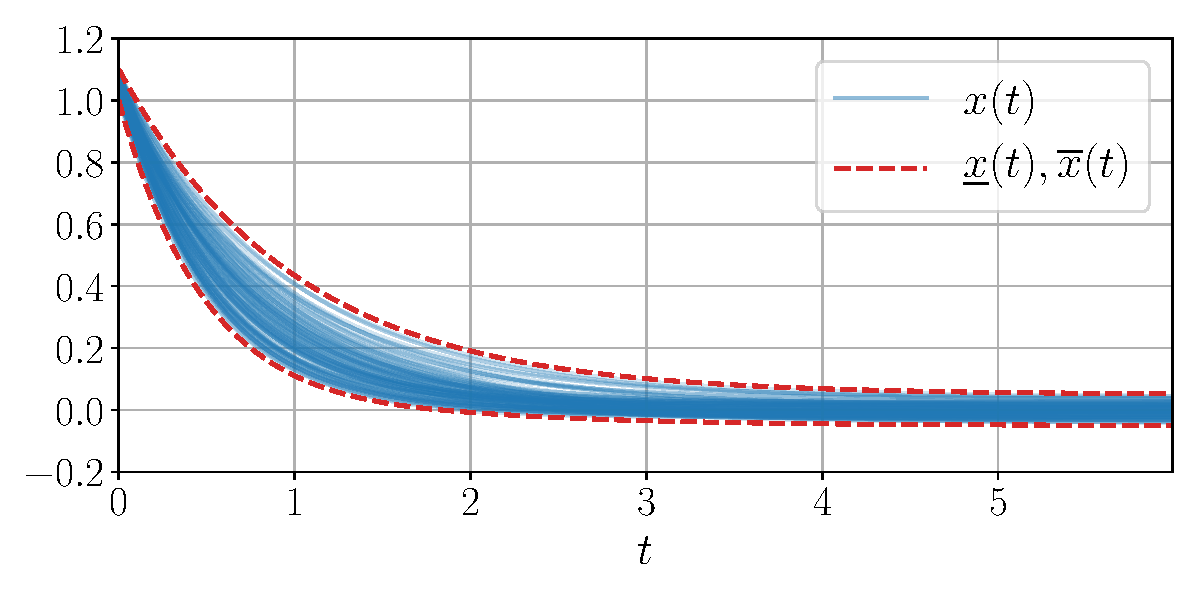
\includegraphics[trim={0 0.6cm 0 0.4cm}, clip, width=\linewidth]{img/interval-predictor}}
    \vspace{-0.7cm}
	\caption{Comparison of \eqref{eq:predictor-naive} and \eqref{eq:interval-predictor} for a simple system \\$\dot{x}(t)=-\theta x(t)+\omega(t)$, with $\theta\in[1, 2]$ and $\omega(t) \in [-0.05, 0.05]$.}
	\label{fig:predictor_example}
\end{figure}

\autoref{fig:predictor_example} illustrates the difference of stability of the two predictors \eqref{eq:predictor-naive} and \eqref{eq:interval-predictor} with a simple example. It suggests to always prefer \eqref{eq:interval-predictor} whenever \autoref{assumpt:metzler} is verified, and only fallback to \eqref{eq:predictor-naive} as a last resort.

% Limitations: set-based method assumes time-varying uncertainty where we have time-invariant uncertainty: $A(\theta)$ is fixed vs $A(\theta)$ can vary in $\cC_\delta$ at each step. Consequence: conservative overset.

\section{Robust Control}

\label{sec:control}
In order to evaluate the robust objective $V^r$ \eqref{eq:robust-control}, we approximate it thanks to the interval prediction $[\underline{x}(t), \overline{x}(t)]$ of \autoref{sec:prediction}.

\begin{definition}[Surrogate objective]
	Let
\begin{align}
\label{eq:surrogate_objective} 
\hat{V}^r(\bu) &\eqdef \sum_{n=N+1}^\infty \gamma^n \underline{R}_n(\bu)\\ 
\text{where}\quad\underline{R}_n(\bu) &\eqdef \min_{x\in[\underline{x}_n(\bu), \overline{x}_n(\bu)]}  R(x) \label{eq:pessimistic-rewards}
\end{align}
and $\underline{x}_n(\bu), \overline{x}_n(\bu)$ follow the dynamics defined in \eqref{eq:interval-predictor}.
\end{definition}

This amounts to changing the reward function, except that the worst case is assessed over the whole past trajectory, which makes this pessimistic reward $\underline{R_n}$ \emph{not markovian}.

\begin{proposition}[Lower bound]
\label{prop:lower-bound}
The surrogate objective  \eqref{eq:surrogate_objective} is a lower bound of the true objective  \eqref{eq:robust-control-disc}: 
\begin{equation*}
\hat{V}^r(\bu) \leq V^r(\bu)
\end{equation*}
\end{proposition}
A direct consequence is that since all our approximations are conservative, if we manage to find a control sequence such that no \textit{``bad event''} (e.g. a collision) happens according to the surrogate objective $\hat{V}^r$, then we are guaranteed that they will not happen either when the controls are executed on the true system. 

\paragraph{Planning}
To optimise $\hat{V}^r$ \eqref{eq:surrogate_objective}, we cannot use Dynamic Programming algorithms since the state space is continuous and the pessimistic rewards are non-markovian. Instead, we turn to tree-based planning algorithms, which optimise a sequence of actions based on the corresponding sequence of rewards, without requiring markovity nor state enumeration. In particular, we consider the \emph{Optimistic Planning of Deterministic Systems} (\texttt{OPD}) algorithm \citep{Hren2008} tailored for the case when the relationship between actions and rewards is deterministic. Indeed, the stochasticity of the perturbations and measurements is encased in $\hat{V}^r$: given the observations up to time $N$ both the predictor dynamics \eqref{eq:interval-predictor} and the pessimistic rewards \eqref{eq:pessimistic-rewards} are deterministic.

At each planning iteration $k\in[K]$, \texttt{OPD} progressively builds a tree $\cT_{k+1}$ by forming upper-bounds $B_a(k)$ over the value of sequences of actions $a$, and expanding\footnote{The expansion of a leaf node $a$ refers to the simulation of its children transitions $aA = \{ab, b\in A\}$} the leaf $a_k$ with highest upper-bound:
\begin{equation}
\label{eq:opd}
a_k = \argmax_{a\in\cL_k} B_a(k), \quad B_a(k) = \sum_{n=0}^{h(a)-1} \underline{R}_n(a) + \frac{\gamma^{h(a)}}{1-\gamma}
\end{equation}
where $\cL_k$ is the set of leaves of $\cT_k$, $h(a)$ is the length of the sequence $a$, and $\underline{R}_n(a)$ the pessimistic reward \eqref{eq:pessimistic-rewards} obtained at time $n$ by following the controls $u_n = \pi_{a_n}(x_n)$.
\begin{theorem}[Planning performance of \citealt{Hren2008}]
\label{theorem:opd-regret}
The simple regret of the \texttt{OPD} algorithm \eqref{eq:opd} applied to the surrogate objective \eqref{eq:surrogate_objective} after $K$ planning iterations is:
\begin{align*}
\text{if } \kappa>1,\quad& 
\hat{V}^r(a^{\star}) - \hat{V}^r({a_K}) = \cO\left(K^{-\frac{\log 1/\gamma}{\log \kappa}}\right);\\
\text{if }\kappa=1,\quad&
\hat{V}^r(a^{\star}) - \hat{V}^r({a_K}) = \cO\left(\gamma^{{(1-\gamma)^{\log_\gamma (\kappa/|\cA|)}}K/{c}}\right)
\end{align*}
where $\kappa$ is a problem-dependent measure of the proportion of near-optimal paths:
\[
\kappa = \limsup_{h\rightarrow\infty} \left|\left\{a\in A^h: \hat{V}^r(a)\geq \hat{V}^r(a^{\star}) - \frac{\gamma^{h+1}}{1-\gamma}\right\}\right|^{1/h}.
\]
\end{theorem}

Hence, by using enough computational budget $K$ for planning we can get as close as we want to the optimal surrogate value $\hat{V}^r(a^{\star})$, at a polynomial rate. Unfortunately, there exists a gap between $\hat{V}^r$ and the true robust objective $V^r$, which stems from three approximations: (i) the true reachable set was approximated by an enclosing interval in \eqref{eq:inclusion-property}; (ii) the time-invariance of the dynamics uncertainty $A(\theta)\in\cC_{[N],\delta}$ was handled by the interval predictor \eqref{eq:interval-predictor} as if it were a time-varying uncertainty $A(\theta(t))\in\cC_{[N],\delta},\forall t$ ; and (iii) the lower-bound $\sum\min\leq \min\sum$ used to define the surrogate objective \eqref{eq:surrogate_objective} is not tight. However, this gap can be bounded with additional assumptions.
\begin{theorem}[Regret bound]
\label{thm:control-error}
Under three conditions:
\begin{enumerate}
	\item a Lipschitz regularity assumption for the reward $R$;
	\item a persistent excitation (PE) assumption:
	\begin{align*}
	\exists \underline{\phi},\overline{\phi}>0: \forall n\geq n_0,\quad \underline{\phi}^2 \leq \lambda_{\min}(\Phi_{n}^\transp\Sigma_{p}^{-1}\Phi_{n}) \leq \overline{\phi}^2;
	\end{align*}
	\item a stability condition: there exist $P>0,Q_0\in\Real^{p\times p}$, $\rho>0$ such that
	$\begin{bmatrix}
		A_0^\transp P + P A_0^\transp + Q_0 & P|D|  \\
		|D|^\transp P & -\rho I_r \\
	\end{bmatrix}< 0;$
\end{enumerate}
 we can bound the approximation error of \autoref{alg:full}:
\begin{equation*}
\hat{V}^r(\bu) \leq {V}^r(\bu) \leq V(\bu) \leq \hat{V}^r(\bu) + \Delta_\omega + \cO\left({\log N / N}\right)
\end{equation*}
with probability at least $1-\delta$, where $\Delta_\omega$ is a constant which corresponds to an irreductible suboptimality suffered from being robust to instantaneous perturbations $\omega(t)$.
\end{theorem}


\section{Multi-model Selection}
\label{sec:multi-model}

The procedure we developed in sections \ref{sec:estimation}, \ref{sec:prediction} and \ref{sec:control} relies on strong modelling assumptions, such as the linear dynamics \eqref{eq:dynamics} and \autoref{assumpt:structure}. But what if they are wrong?

\paragraph{Model adequacy}

One of the major benefits of using the family of linear models, compared to richer model classes, is that they provide strict conditions allowing to quantify the adequacy of the modelling assumptions to the observations.

Given $N-1$ observations, \autoref{sec:estimation} provides a polytopic confidence region \eqref{eq:polytope} that contains $A(\theta)$ with probability at least $1-\delta$. Since the dynamics are linear, we can propagate this confidence region to the next observation: $y_{N}$ must belong to the Minkowski sum of a polytope representing model uncertainty $\cP(A_{0} x_N + Bu_N, \Delta A_{1}x_N,\dots, \Delta A_{2^d}x_N)$ and a polytope $\cP(0_p, \underline{\eta}, \overline{\eta})$ bounding the perturbation and measurement noises. \citet{delos2015} provide a way to test this membership in polynomial time using linear programming. Whenever it is not verified, we can confidently reject the $(A,\phi)$-modelling \autoref{assumpt:structure}. This enables us to consider a rich set of potential features $\left((A^1, \phi^1), \dots, (A^M, \phi^M)\right)$ rather than relying on a single assumption, and only retain those that are consistent with the observations so far. Then, every remaining hypothesis must be considered during planning.

\paragraph{Robust selection}

We temporarily ignore the parametric uncertainty on $\theta$ to simply consider several candidate dynamics models, which all correspond to different modelling assumptions. We also restrict to deterministic dynamics, which is the case of \eqref{eq:interval-predictor}.

\begin{assumption}[Multi-model ambiguity]
\label{assumpt:multi-model-ambiguity}
The true dynamics $f$ lies within a finite set of candidate models $f^1, \dots, f^M$.
\begin{equation*}
\exists m\in[M]: \dot{x}(t) = f^m(x(t), u(t)), \forall t\geq 0
\end{equation*}
\end{assumption}
We want to adapt our planning algorithm in order to balance these concurrent hypotheses in a robust fashion, i.e. maximise a robust objective with discrete ambiguity:
\begin{equation}
\label{eq:robust-objective-discrete}
V^r = \sup_{a\in\cA^\Natural}\min_{m\in[M]} \sum_{n=N+1}^\infty \gamma^n R_n^m
\end{equation}
where $R_n^m$ is the reward obtain by following the action sequence $a$ up to step $n$ under the dynamics $f^m$.
This objective could be optimised in the same way as in \autoref{sec:control}, but this would result in a coarse and lossy approximation. Instead, we exploit the finite uncertainty structure of \autoref{assumpt:multi-model-ambiguity} to asymptotically recover the true $V^r$ by modifying the \texttt{OPD} algorithm in the following way:

\begin{definition}[Robust sequence upper bounds] We replace the upper-bound \eqref{eq:opd} on sequence values in \texttt{OPD} by:
\begin{equation}
\label{eq:robust-b-values}
B_a^r(k)  \eqdef \min_{m\in[M]} \sum_{n=0}^{h-1} \gamma^n R_n^m  + \frac{\gamma^h}{1-\gamma}
\end{equation}
\end{definition}
An illustration of the computation of the robust upper-bounds is presented in Figure \ref{fig:drop}. Note that it is not equivalent to solving each control problem independently and following the action with highest worst-case value, as we show in the Supplementary Material. We analyse the sample complexity of the corresponding robust planning algorithm.

\begin{figure}
\centering
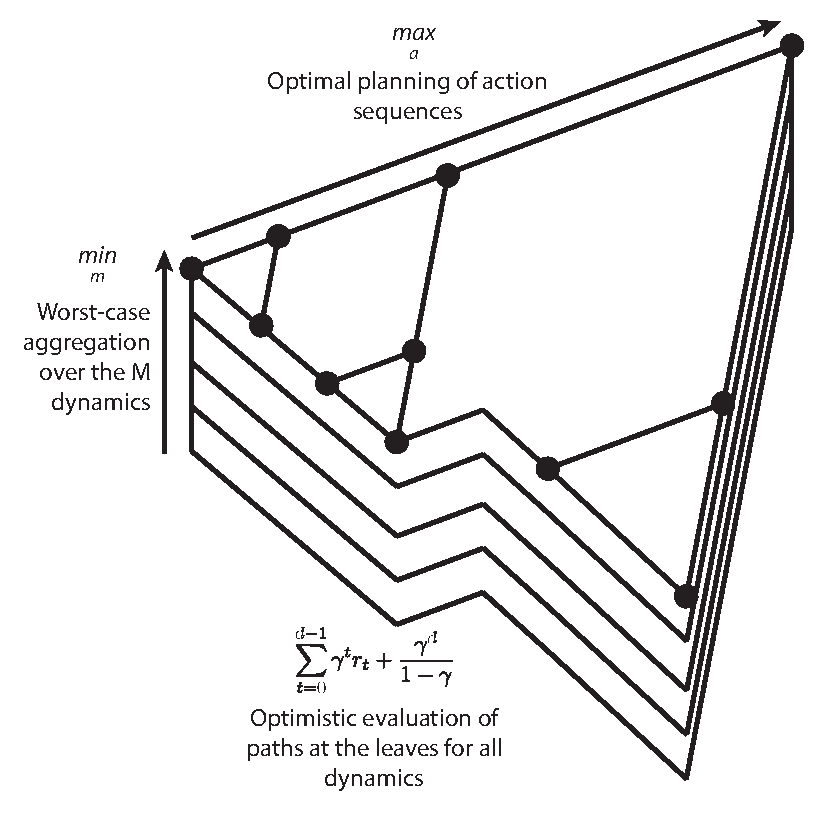
\includegraphics[width=0.4\linewidth]{img/robust-control-tree}
\caption{The computation of robust B-values in \eqref{eq:robust-b-values}. The simulation of trajectories for every dynamics model $f^m$ is represented as stacked versions of the expanded tree $\mathcal{T}_k$.}
\label{fig:drop}
\end{figure}

\begin{theorem}[Robust planning performance]
\label{theorem:drop-regret}
The robust version of \texttt{OPD} \eqref{eq:robust-b-values} enjoys the same regret bound as \texttt{OPD} in \autoref{theorem:opd-regret}, with respect to the multi-model objective \eqref{eq:robust-objective-discrete}.
\end{theorem}

The regret depends on the number $K$ of node expansions, but each expansion now requires $M$ times more simulations than in the single-model setting. The solution of the robust objective \eqref{eq:robust-objective-discrete} with discrete ambiguity $f\in\{f^m\}_{m\in[M]}$ can be recovered exactly, asymptotically when the planning budget $K$ goes to infinity. This contrasts the results obtained in \autoref{sec:control} for the robust objective \eqref{eq:robust-control} with continuous ambiguity $A(\theta)\in\cC_{[N],\delta}$, for which \texttt{OPD} only recovers the surrogate approximation $\hat{V}^r$, as discussed in \autoref{thm:control-error}. Finally, the two approaches of Sections \ref{sec:control} and \ref{sec:multi-model} can be merged by using the pessimistic reward \eqref{eq:pessimistic-rewards} in \eqref{eq:robust-b-values}.

\section{Experiments}
\label{sec:experiments}

\paragraph{Obstacle avoidance with unknown friction}
We first consider a simple illustrative example, shown in \autoref{fig:prediction}: the control of a 2D system with position $(p_x,p_y)$ and velocity $(v_x, v_y)$ moving by means of a force $(u_x, u_y)$ in an environment with unknown anisotropic friction.

\begin{equation*}
\begin{bmatrix}
\dot{p_x}\\
\dot{p_y}\\
\dot{v_x}\\
\dot{v_y}\\
\end{bmatrix} = 
\begin{bmatrix}
0 & 0 & 1 & 0 \\
0 & 0 & 0 & 1 \\
0 & 0 & -\theta_x & 0 \\
0 & 0 & 0 & -\theta_y
\end{bmatrix}
\begin{bmatrix}
{p_x}\\
{p_y}\\
{v_x}\\
{v_y}\\
\end{bmatrix}
+
\begin{bmatrix}
0\\
0\\
{u_x}\\
{u_y}\\
\end{bmatrix}
\end{equation*}

Note that \autoref{assumpt:metzler} is always verified. The reward is non-smooth and encodes the task of navigating to reach a goal state $x_g$ while avoiding collisions with obstacles: $R(x) = \delta(x)/(1 + \|x - x_g\|_2)$  where $\delta(x)$ is $0$ whenever $x$ collides with an obstacle, $1$ otherwise. The actions $\cA$ are constant controls in the up, down, left and right directions.

We run \autoref{alg:full} for 100 simulations, and compare in \autoref{tab:obstacle} its performances to that of the nominal agent, i.e. the non-robust adaptive control approach that plans with the estimated dynamics $\theta_{[N],\lambda}$. We observe that though the robust agent performs worse than the nominal agent on average, it manages to ensure safety and attains a better worst-case performance, as intended. We also study the evolution of the simple regret $V(x_n) - J_n(x_n)$ with respect to the number of samples $N$, where $J_n(x_n) = \sum_{i > n} \gamma^i R_i$ is the empirical return at state $x_n$ in a trajectory $x_0, R_0, x_1, R_1, \dots$, while $V(x_n)$ is the optimal value that the agent would get by acting optimally from $x_n$ with knowledge of the dynamics. The mean regret is shown in \autoref{fig:regret}, along with its 95\% confidence interval. We see that \autoref{alg:full} has a regret $\hat{V}^r - V$ decreasing at least polynomially with $N$, as expected from \autoref{thm:control-error}. This shows that the agent gets more aggressive when it is more confident, as desired, while ensuring safety at all time. In contrast, the nominal agent has an even smaller regret but collided with obstacles in $4\%$ of simulations.

\begin{figure}[tp]
	\centering
	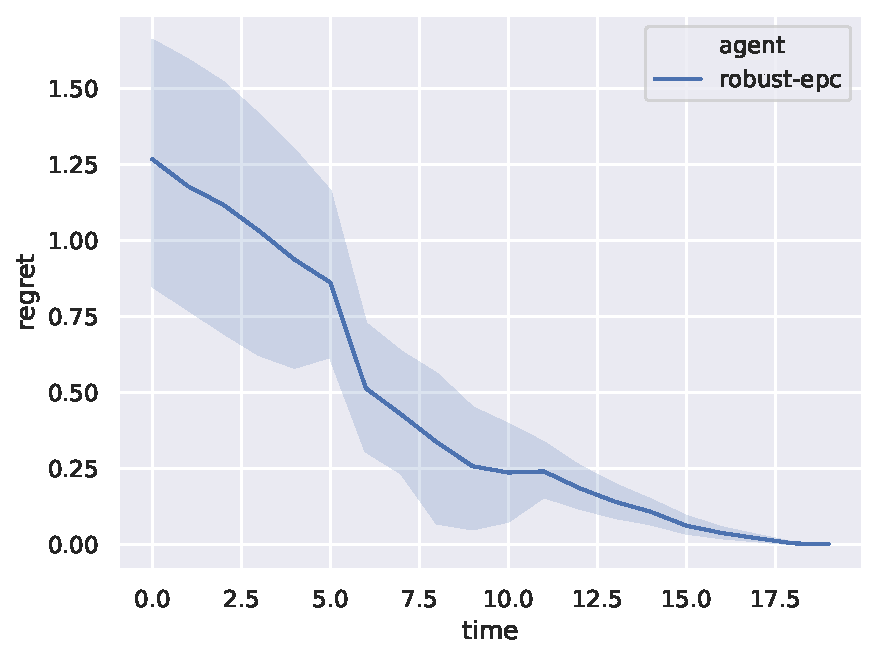
\includegraphics[width=0.8\linewidth]{img/regret.pdf}
	\caption{The mean regret along with its $95\%$ confidence interval with respect to $N$, for the robust and nominal agents.}
	\label{fig:regret}
\end{figure}

\begin{table}[tbp]
	\caption{Performances on the obstacle avoidance task}
	\label{tab:obstacle}
	\centering
	\begin{tabular}{lccc}
		\toprule
		Agent &
		failures &
		min return &
		mean return $\pm$ std  \\
		\midrule
		Oracle & 0\% & {11.6} & {$14.2 \pm 1.3$} \\
		\midrule
		{Nominal} & {4\%} & {2.8} & \textbf{$\mathbf{13.8} \pm 2.0$} \\
		\autoref{alg:full} & \textbf{0\%} & \textbf{10.4} & {$13.0 \pm 1.5$} \\
		\bottomrule
	\end{tabular}
\end{table}

\paragraph{Behavioural planning for an autonomous vehicle}
We consider the \href{https://github.com/eleurent/highway-env}{highway-env} environment \citep{highway-env} for simulated driving decision problems. An autonomous vehicle with state $\chi_0\in\Real^4$ is approaching an intersection among $V$ other vehicles with states $\chi_i\in\Real^4$, resulting in a joint traffic state $x = [\chi_0, \dots,\chi_V]^\top\in\Real^{4V+4}$. These vehicles follow parametrized behaviours $\dot{\chi}_i=f_i(x,\theta_i)$ with unknown parameters $\theta_i\in\Real^5$. We appreciate a first advantage of the structure imposed in \autoref{assumpt:structure}: the uncertainty space of $\theta$ is $\Real^{5V}$. In comparison, the traditional LQ setting where the whole state matrix $A$ is estimated would have resulted in a much larger parameter space $\theta\in\Real^{16V^2}$.
%This allows to scale to larger systems: in our experiments, we used a state space of dimension $44$ ($V=10$) where e.g. \citep{Dean2018,abeille18a} reported numerical experiments with states of dimensions 3 and 4, respectively.
The system dynamics $f$, which describes the couplings and interactions between vehicles, can only be expressed in the form of \autoref{assumpt:structure} given the knowledge of the desired route for each vehicle, with features $\phi$ expressing deviations to the centerline of the followed lane. Since these intentions are unknown to the agent, we adopt the multi-model perspective of \autoref{sec:multi-model} and consider one model per possible route for every observed vehicle before an intersection. We compare \autoref{alg:full} to a nominal agent planning with the estimated parameter $\theta_{[N],\lambda}$, with two different modelling assumptions: we assume that Nominal 1 has access to the true followed route for each vehicle, while Nominal 2 does not and picks a model with minimal prediction error. There performances are compared in \autoref{tab:driving}. Again, the robust approach is less efficient on average than planning with a nominal model, but it does better in terms of worst-case performance and manages to avoid collisions, contrary to the nominal baselines that suffer from model bias. We provide more details about the system and videos of the experiments in the Supplementary Material.

\begin{figure}[t]
	\centering
	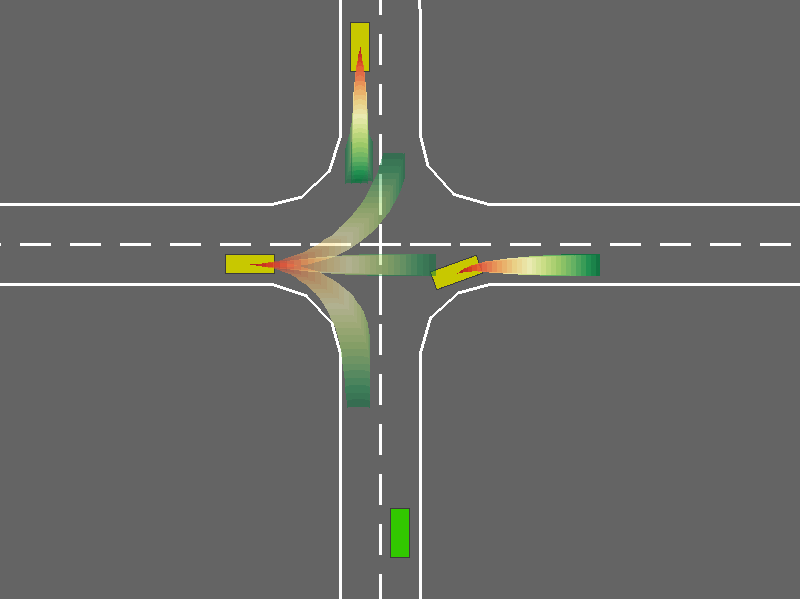
\includegraphics[width=0.7\linewidth]{img/highway-small}
	\caption{The intersection crossing task. We show the trajectory intervals corresponding to behavioural uncertainty for each observed vehicle, and the multi-model assumption over the followed route.}
\end{figure}

\begin{table}[t]
	\caption{Performances on the driving task}
	\label{tab:driving}
	\centering
	\begin{tabular}{lccc}
		\toprule
		Agent &
		failures &
        min return &
		mean return $\pm$ std  \\
		\midrule
		Oracle & 0\% & {6.9} & $7.4 \pm 0.5$ \\
		\midrule
		{Nominal 1} & 4\% & {5.2} & $\mathbf{7.3} \pm 1.5$ \\
		{Nominal 2} & 33\% & {3.5} & $6.4 \pm 0.26$ \\
		\autoref{alg:full} & \textbf{0\%} & \textbf{6.8} & $7.1 \pm 0.29$ \\
		\bottomrule
	\end{tabular}
\end{table}

\section*{Conclusion}

We present a framework for the robust estimation, prediction and control of a partially known linear system with generic costs. Leveraging tools from linear regression, interval prediction, and tree-based planning, we guarantee the predicted performance for the true system and provide a regret bound. The applicability of the method is further improved by a multi-model extension, and demonstrated on two simulated applications.

\clearpage
\bibliography{references}
\bibliographystyle{icml2020}

\clearpage
\onecolumn
\appendix

\begin{center}
	\LARGE Supplementary Material
\end{center}

\paragraph{Outline}
In \autoref{sec:proof}, we provide a proof for every novel result introduced in this paper. \autoref{sec:tight-polytope} describes a better method of conversion from ellipsoid to polytope than that of \eqref{eq:polytope}. \autoref{sec:min-max-order} highlights the fact that robustness cannot be recovered by aggregating independent solutions to many optimal control problem. Finally, \autoref{sec:experimental-setting} gives additional details on the setting of our experiments.

\section{Proofs}
\label{sec:proof}

\subsection{Proof of \autoref{prop:regularized_solution}}

\begin{proof}
We differentiate $J(\theta) = \sum_{n=1}^N \|y_n -\Phi_n\theta\|_{\Sigma_p^{-1}}^2 + \lambda\|\theta\|_{}^2$ as in  \eqref{eq:regression_min} with respect to $\theta$:

\begin{align*}
    \nabla_{\theta} J(\theta) &= \sum_{n=1}^N\nabla_{\theta} (y_n - \Phi_n\theta)^\transp\Sigma_p^{-1}(y_n - \Phi_n\theta) + \nabla_{\theta} \lambda\|\theta\|_{}^2\\
    &= -2\sum_{n=1}^N y_n^\transp\Sigma_p^{-1}\Phi_n + 2\sum_{n=1}^N\theta^\transp(\Phi_n^\transp\Sigma^{-1}\Phi_n) +  2 \lambda \theta^\transp
\end{align*}

Hence,
\begin{align*}
    \nabla_{\theta} J(\theta) = 0 \iff \left(\sum_{n=1}^N\Phi_n^\transp\Sigma_p^{-1}\Phi_n + I_d\right)\theta = \sum_{n=1}^N y_n^\transp\Sigma_p^{-1}\Phi_n
\end{align*}
\end{proof}

\subsection{Proof of \autoref{thm:confidence_ellipsoid}}

We start by showing a preliminary proposition:

\begin{proposition}[Matrix version of Theorem 1 of \citealt{Abbasi2011}]
\label{prop:concentration}
Let $\{F_n\}_{n=0}$ be a filtration.
Let $\{\eta_n\}_{n=1}^\infty$ be a $\Real^p$-valued stochastic process such that $\eta_n$ is $F_n$-measurable and $\expectedvalue\left[\eta_n\condbar F_{n-1}\right]$ is $\Sigma_p$-sub-Gaussian.

Let $\{\Phi_n\}_{n=1}^\infty$ be an $\Real^{p\times d}$-valued stochastic process such that $\Phi_n$ is $F_n$-measurable. Assume that $G$ is a $d\times d$ positive definite matrix. For any $n\geq 0$, define:
\begin{equation*}
    \overline{G}_n = G + \sum_{s=1}^n \Phi_s^\transp \Sigma_p^{-1} \Phi_s \in \Real^{d\times d} \quad S_n = \sum_{s=1}^n \Phi_s^\transp\Sigma_p^{-1}\eta_s \in \Real^{d}.
\end{equation*}
Then, for any $\delta>0$, with probability at least $1-\delta$, for all $n\geq0$,
\begin{align*}
\| S_n \|_{\overline{G}_n^{-1}} \geq \sqrt{2\ln \left(\frac{\det\left(\overline{G}_n\right)^{1/2}}{\delta\det(G)^{1/2}}\right)}.
\end{align*}
\end{proposition}
\begin{proof}
Let 
\begin{equation*}
    G_t = \sum_{s=1}^t \Phi_s^\transp \Sigma_p^{-1} \Phi_s \in \Real^{d\times d}
\end{equation*}
And for any $z\in\Real^d$,
\begin{equation*}
    M_t^z = \exp{\left(\inp{z}{S_t} - \frac{1}{2}\|z\|_{G_t}\right)}
\end{equation*}
\begin{equation*}
    D_t^z = \exp{\left(\inp{\Phi_t z}{\eta_t}_{\Sigma_p^{-1}} - \frac{1}{2}\|\Phi_t z\|_{\Sigma_p^{-1}}\right)}
\end{equation*}
Then,
\begin{align*}
    M_t^z &= \exp{\left(\sum_{s=1}^t z^\transp \Phi_s^\transp \Sigma_p^{-1} \eta_s - \frac{1}{2} (\Phi_s z)^\transp\Sigma_p^{-1}(\Phi_s z) \right)} \\
    &= \prod_{s=1}^{t} D_s^z
\end{align*}
and using the Sub-Gaussianity of $\eta_t$
\begin{align*}
    \expectedvalue\left[D_t^z \condbar F_{t-1}\right] = {}& \exp{\left(- \frac{1}{2}\|\Phi_t z\|_{\Sigma_p^{-1}}\right)}\\ &\expectedvalue\left[\exp{\left(\inp{\Phi_t z}{\eta_t}_{\Sigma_p^{-1}}\right)} \condbar F_{t-1}\right]  \\
    \leq {} & \exp{\left(- \frac{1}{2}\|\Phi_t z\|_{\Sigma_p^{-1}}\right)}\\
    &\exp{\left((z^\transp \Phi_t^\transp \Sigma_p^{-1})\Sigma_p(\Sigma_p^{-1} \Phi_t z)\right)}\\
    &= 1
\end{align*}
\begin{align*}
    \expectedvalue\left[M_t^z \condbar F_{t-1}\right] = \left(\prod_{s=1}^{t-1} D_s^z\right) \expectedvalue\left[D_t^z \condbar F_{t-1}\right] \leq M_{t-1}^z
\end{align*}
Showing that $(M_t^z)_{t=1}^\infty$ is indeed a supermartingale and in fact $\expectedvalue[M_t^z]\leq 1$.
It then follows by Doob's upcrossing lemma for supermartingale that $M_\infty^z = \lim_{t\to\infty} M_t^z$ is almost surely well-defined, and so is $M_\tau^z$ for any random stopping time $\tau$.

Next, we consider the stopped martingale $M_{\min(\tau,t)}^z$. Since 
$(M_t^z)_{t=1}^\infty$ is a non-negative supermartingale and $\tau$ is a random stopping time, we deduce by Doob's decomposition that
\begin{align*}
\expectedvalue[M_{\min(\tau,t)}^z] &= \expectedvalue[M_0^z] + \expectedvalue[\sum_{s=0}^{t-1} (M_{s+1}^z-M_s^z) \mathbb{I}\{\tau>s\}]\\
&\leq 1 + \expectedvalue[\sum_{s=0}^{t-1} \expectedvalue[M_{s+1}^z-M_s^z|F_{s}] \mathbb{I}\{\tau>s\}]\\
&\leq 1
\end{align*}
Finally, an application of Fatou's lemma show that 
$\expectedvalue[M_\tau^z] = \expectedvalue[\liminf_{t\to\infty} M_{\min(\tau,t)}^z] \leq \liminf_{t\to\infty} \expectedvalue[M_{\min(\tau,t)}^z] \leq 1.$

This results allows to apply a result from \citep{pena2008self}:
\begin{lemma}[Theorem 14.7 of \citep{pena2008self}]
If $Z$ is a random vector and $B$ is a symmetric positive definite matrix such that
\[\forall \gamma\in\Real^d, \ln \expectedvalue \exp \left(\gamma^\transp Z -\frac{1}{2} \gamma^\transp B \gamma \right)\leq 0,\]
then for any positive definite non-random matrix C, it holds
\[\expectedvalue\left[ \sqrt{\frac{\det(C)}{\det(B+C)} } \exp\left( \frac{1}{2}\|Z\|^2_{(B+C)^{-1}}\right)\right]\leq 1. \] 
In particular, by Markov inequality, for all $\delta\in(0,1)$, 
\[\probability{\|Z\|_{(B+C)^{-1}} \geq \sqrt{2\ln \left(\frac{\det \left((B+C)^{1/2}\right)}{\delta\det(C)^{1/2}}\right)}}\leq \delta.\]
\end{lemma}

Here, by using $Z = \sum_{s=1}^t\Phi_s\Sigma_p^{-1}\eta_s$, $B=G_t$, $C=G$,

\[
\probability{\| S_t \|_{(G_t+G)^{-1}} \geq \sqrt{2\ln \left(\frac{\det(G_t+G)^{1/2}}{\delta\det(G)^{1/2}}\right)}} \leq \delta
\]

\end{proof}

Having shown this preliminary result, we move on to the proof of \autoref{thm:confidence_ellipsoid}.

\begin{proof}
For all $x\in\Real^d$, \eqref{eq:vector_rls} gives:
\begin{align*}
    x^\transp\theta_{N,\lambda}  -x^\transp\theta &= x^\transp G_{N, \lambda}^{-1}\sum_{n=1}^N \Phi_n^\transp \Sigma_p^{-1}\eta_n
    - \lambda x^\transp G_{N, \lambda}^{-1}\theta\\
    &= \inp{x}{\sum_{n=1}^N \Phi_n^\transp \Sigma_p^{-1}\eta_n}_{G_{N, \lambda}^{-1}} - \lambda\inp{x}{\theta}_{G_{N, \lambda}^{-1}}
\end{align*}

Using the Cauchy-Schwartz inequality, we get:
\begin{align*}
    |x^\transp\theta_{N,\lambda}  -x^\transp\theta| \leq {} & \|x\|_{G_{N, \lambda}^{-1}}\left(\left\|\sum_{n=1}^N \Phi_n^\transp \Sigma_p^{-1}\eta_n\right\|_{G_{N, \lambda}^{-1}}\right.\\ 
    &+ \left.\lambda\|\theta\|_{G_{N, \lambda}^{-1}}\right)
\end{align*}

In particular, for $x = G_{N,\lambda}(\theta_{N,\lambda} - \theta)$, we get after simplifying with $\| \theta_{N,\lambda}  - \theta\|_{G_{N,\lambda}}$:
\begin{align*}
    \| \theta_{N,\lambda}  - \theta\|_{G_{N,\lambda}} &\leq \left\|\sum_{n=1}^N \Phi_n^\transp \Sigma_p^{-1}\eta_n\right\|_{G_{N, \lambda}^{-1}} + \lambda\|\theta\|_{G_{N, \lambda}^{-1}}
\end{align*}

By applying \autoref{prop:concentration} with $G=\lambda I_d$, we obtain that with probability at least $1-\delta$,
\begin{align*}
    \| \theta_{N,\lambda}  - \theta\|_{G_{N,\lambda}} &\leq \sqrt{2\ln \left(\frac{\det(G_{N,\lambda})^{1/2}}{\delta\det(\lambda I_d)^{1/2}}\right)}
     + \lambda\|\theta\|_{G_{N, \lambda}^{-1}}
\end{align*}
And since $\|\theta\|_{G_{N, \lambda}^{-1}}^2 \leq 1/\lambda_{\min}(G_{N,\lambda})\|\theta\|_2^2 \leq 1/\lambda \|\theta\|_2^2$ and $\|\theta\|_2^2 \leq d\|\theta\|_\infty^2\leq d S^2$,
\begin{align*}
    \| \theta_{N,\lambda}  - \theta\|_{G_{N,\lambda}} &\leq \sqrt{2\ln \left(\frac{\det(G_{N,\lambda})^{1/2}}{\delta\det(\lambda I_d)^{1/2}}\right)}
     + (\lambda d)^{1/2}S
\end{align*}
\end{proof}


\subsection{Proof of \autoref{prop:lower-bound}}

\begin{proof}
	The predictor designed in \autoref{sec:prediction} verifies the inclusion property \eqref{eq:inclusion-property}. Thus, for sequence of controls $\bu$, any dynamics $A(\theta)\in C_{[N],\delta}$, and perturbations $\underline{\bom} \leq \bom \leq \overline{\bom}$, the corresponding state at time $t_n$ is bounded by $\underline{x}_n \leq x_n \leq \overline{x}_n$, which implies that $R(x_n) \geq \min_{x\in[\underline{x}_n(\bu), \overline{x}_n(\bu)]}  R(x) = \underline{R}_n(\bu)$.
	
	Thus, by taking the min over $C_{[N],\delta}$ and $[\underline{\bom}, \overline{\bom}]$, we also have for any sequence of controls $\bu$:
	\begin{align*}
	    V^r(\bu) &= \min_{\substack{A(\theta)\in C_{[N],\delta}\\ \underline{\bom} \leq \bom \leq \overline{\bom}}} \sum_{n=N+1}^\infty \gamma^n R(x_n)\\
	    &\geq \sum_{n=N+1}^\infty \gamma^n \underline{R}_n(\bu)\\
	    &= \hat{V}^r(\bu)
	\end{align*}
\end{proof}

\subsection{Proof of \autoref{thm:control-error}}

We first bound the model estimation error.
\begin{lemma}
If the features $\Phi_n$ are persistently exciting:
\begin{align}
\label{eq:excitation}
\exists \underline{\phi},\overline{\phi}>0, n_0: \forall n\geq n_0,\nonumber\\ \underline{\phi}^2 \leq \lambda_{\min}(\Phi_{n}^\transp\Sigma_{p}^{-1}\Phi_{n}) \leq \overline{\phi}^2,
\end{align}
then,
\[\|A(\theta) - A(\theta_{[N],\lambda})\|_2 = \cO\left( \sqrt{\frac{\log N}{N}} \right) \]
\end{lemma}
\begin{proof}
By \eqref{eq:g_n_lambda} and \eqref{eq:excitation}, we have $$\lambda_{\min}(G_{[N],\lambda,i,j}) \geq (N-n_0)\underline{\phi}^2 + \sum_{n<n_0}\Phi_{n}^\transp\Sigma_{p}^{-1}\Phi_{n}$$

Hence, by \eqref{eq:confidence-ellipsoid} we have 
\begin{align*}
	\|\theta - \theta_{[N],\lambda}\|_{G_{[N],\lambda}} \geq (\sqrt{N}\underline{\phi} + \cO(1))\|\theta - \theta_{[N],\lambda}\|_{2}
\end{align*}
and \eqref{eq:beta_n} gives

\begin{align*}
\beta_N(\delta) &= \sqrt{2\ln \left(\frac{\det(G_{N,\lambda})^{1/2}}{\delta\det(\lambda I_d)^{1/2}}\right)}
+ (\lambda d)^{1/2}S\\
&\leq \sqrt{d\log (N\overline{\phi}^2) / \lambda^{d/2}} + \cO(1)
\end{align*}
Thus,
\[\|\theta - \theta_{[N],\lambda}\|_{2} = \cO\left( \sqrt{\frac{\log N}{N}} \right) \]

And $A(\theta)$ belongs to a linear image of this $L^2$-ball. By writing a the $j^{th}$ column of a matrix $M$ as $M_j$, and its coefficient $i,j$ as $M_{i,j}$,
\begin{align*}
((A(\theta)&-A(\theta_{[N],\lambda}))^\transp (A(\theta) - A(\theta_{[N],\lambda})))_{i,j}\\
%&= (\phi_i(\theta-\theta_{[N],\lambda}))^\transp \phi_j(\theta-\theta_{[N],\lambda}) \\
&= (\theta-\theta_{[N],\lambda})^\transp\phi_{i}^{\transp}\phi_j(\theta-\theta_{[N],\lambda}) \\
&\leq \lambda_{\max}(\phi_{i}^{\transp}\phi_j) \|\theta - \theta_{[N],\lambda}\|_{2}^2 = \cO\left( {\frac{\log N}{N}} \right) 
\end{align*}

\end{proof}

Then, we propagate this estimation error through the state prediction.

\begin{lemma}
If there exist $P>0,Q_0\in\Real^{p\times p}$, $\rho>0$ such that
\begin{align*}
\begin{bmatrix}
A_0^\transp P + P A_0^\transp + Q_0 & P|D|  \\
|D|^\transp P & -\rho I_r \\
\end{bmatrix}< 0,
\end{align*}
then for all $t> t_N$,
\[\|\ox(t) - \ux(t)\| \leq \left(C_0 + \cO\left({\frac{\log N}{N}} \right)\right)C_\omega(t) \]
where $C_\omega(t) = \sup_{\tau\in[t_N,t]} \|\overline{\omega}(\tau) - \underline{\omega}(\tau)\|_2^2$ and $C_0 = \sqrt{{2\rho\lambda_{\max}(P)}/({\lambda_{\min}(P)\lambda_{\min}(Q_0)})}$.
\end{lemma}
\begin{proof}
Let $e = \ox - \ux$. \eqref{eq:interval-predictor} gives the dynamics:
\begin{align*}
\dot{e} = A_0e + |\Delta A|(\ox^+ + \ux^-) + |D|(\overline{\omega} - \underline{\omega})
\end{align*}
where recall that $|M| = M^+ + M^-$ for any matrix $M\in\Real^{p\times p}$.

We define the Lyapunov function $V = e^\transp P e$, which is non-negative definite provided that
$
P>0,
$ and compute its derivative:
\begin{align*}
\dot{V} ={}& X^\transp
\begin{bmatrix}
A_0^\transp P + P A_0^\transp + Q & P|D| & P|\Delta A| \\
|D|^\transp P & -\rho I_r & 0\\
|\Delta A|^\transp P & 0 & -\alpha I_p
\end{bmatrix}
X\\
& - e^\transp Q e + \alpha |\ux^+ + \ox^-|^2 + \rho |\overline{\omega} - \underline{\omega}|^2
\end{align*}
with $X=\begin{bmatrix}
e & \overline{\omega} - \underline{\omega} &  \ux^+ + \ox^-
\end{bmatrix}^\transp$, for any $Q\in\Real^{p\times p}$, $\rho,\alpha\in\Real$ . 

Moreover, it holds that $-\ux^+ -\ox^- \leq e \leq \ox^+ + \ux^-$, which implies $|\ux^+ + \ox^-| \leq 2 |e|$. Hence,
\begin{align*}
\dot{V} \leq {}& X^\transp
\underbrace{
\left[
\begin{array}{cc|c}
A_0^\transp P + P A_0^\transp + Q + 4\alpha I_p & P|D| & P|\Delta A| \\
|D|^\transp P & -\rho I_r & 0\\
\hline
|\Delta A|^\transp P & 0 & -\alpha I_p
\end{array}
\right]}_{\Upsilon}
X\\
& - e^\transp Q e + \rho \|\overline{\omega} - \underline{\omega}\|_2^2
\end{align*}

Thus, if we had $\Upsilon \leq 0$, $Q>0$, $\rho > 0$, then we would have
\[
\dot{V} \leq -\mu V + \rho \|\overline{\omega} - \underline{\omega}\|_2^2
\]
with $\mu = \frac{\lambda_{\min}(Q)}{\lambda_{\max}(P)}$. Since $V(t_N) = 0$, this further implies that for all $t>t_N$, 
\begin{equation}
\label{eq:lyap-bound}
V(t) \leq \frac{\rho}{\mu} C_\omega(t)
\end{equation}

We now examine the condition $\Upsilon \leq 0$.
We resort to its Schur complement: given $\alpha > 0$ , $\Upsilon \leq 0$ if and only if $R \geq S$, where $S= \alpha^{-1}\begin{bmatrix}|\Delta A|^\transp P & 0\end{bmatrix}^\transp \begin{bmatrix}|\Delta A|^\transp P & 0\end{bmatrix}$ and $R$ is the top-left block of $-\Upsilon$:
\[R = \begin{bmatrix}
-A_0^\transp P - P A_0^\transp - Q - 4\alpha I_p & -P|D|\\
-|D|^\transp P & \rho I_r\\
\end{bmatrix}\]

Choose $Q = \frac{1}{2}Q_0-4\alpha I_p$.
Assume that $P$ is fixed and satisfies the conditions of the lemma. We have $$\lambda_{\max}(S) \leq \alpha^{-1}\lambda_{\max}(|\Delta A|)^2\lambda_{\max}(P)^2.$$

Thus, by taking $\alpha = \frac{\lambda_{\max}(|\Delta A|)^2\lambda_{\max}(P)^2}{2\lambda_{\min}(Q_0)} = \cO(\log N / N)$, we can obtain that $S \leq \begin{bmatrix}
\frac{1}{2}Q_0 & 0\\0 & 0
\end{bmatrix}$. Thus,
\[R-S \geq \begin{bmatrix}
-A_0^\transp P - P A_0^\transp - Q_0 & -P|D|\\
-|D|^\transp P & \rho I_r\\
\end{bmatrix} > 0 \]
as it is assumed in the conditions of the lemma. Hence, under such a choice of $\alpha$ and $Q$, we recover $\Upsilon\leq 0$. \eqref{eq:lyap-bound} follows with $\mu = \frac{\lambda_{\min}(Q)}{\lambda_{\max}(P)} = \frac{\frac{1}{2}\lambda_{\min}(Q_0) - 4\alpha}{\lambda_{\max}(P)}$.
Finally, we obtain
\begin{align*}
\|e(t)\|_2^2 &\leq \lambda_{\min}(P)^{-1} V(t)\\
& \leq \frac{2\rho\lambda_{\max}(P)/\lambda_{\min}(P)}{\lambda_{\min}(Q_0) - 8\alpha} C_\omega(t)\\
\end{align*}
Developing at the first order in $\alpha$ gives
\begin{align*}
\|e(t)\|_2 &\leq C_0\left(1 + \frac{4\alpha}{\lambda_{\min}(Q_0)} + \cO(\alpha_N^2)\right)C_\omega(t)\\
&\leq \left(C_0 + \cO(\log N/N)\right)C_\omega(t)
\end{align*}
\end{proof}


Finally, we propagate the state prediction error bound to the pessimistic rewards and surrogate objective to get our final result.
\begin{proof}
  
 For any sequence of controls $\bu$, dynamics $A(\theta)\in C_{[N],\delta}$ and perturbations $\underline{\bom} \leq \bom \leq \overline{\bom}$, we clearly have 
 \[V(\bu)^r \leq V(\bu) = \expectedvalue_{\bom}\sum_n \gamma^n R(x_n)\]
 
 Moreover, by the inclusion property \eqref{eq:inclusion-property}, we have that $\underline{x}_n \leq x_n \leq \overline{x}_n$, which implies that $R(x_n) \leq \max_{x\in[\underline{x}_n(\bu), \overline{x}_n(\bu)]}  R(x)$. Assuming $R$ is $L$-lipschitz,
 \begin{align*}
     V(\bu) - \hat{V}^r(\bu) &\leq \sum_{n=N+1}^\infty \gamma^n \underset{{x\in[\underline{x}_n(\bu), \overline{x}_n(\bu)]}}{(\max - \min)} R(x)\\
     &\leq \sum_{n=N+1}^\infty \gamma^n L \left\|\underline{x}_n(\bu) - \overline{x}_n(\bu)\right\|_2\\
     &\leq L(C_0 + \cO\left({\log N / N}\right)) \sum_{n>N} \gamma^n C_{\omega}(t_n)\\
     &= \Delta_\omega + \cO\left({\log N / N}\right)
 \end{align*}
 with $\Delta_\omega = L C_0\sum_{n>N} \gamma^n C_{\omega}(t_n)$.
 
 Note that $\Delta_\omega$ is finite, since $C_{\omega}(t_n)$ is in the order of $\underline{\omega}(t_n)$, $\overline{\omega}(t_n)$, and these are either bounded in the case of \autoref{assumpt:bounded-noise}, or in the case of \autoref{assumpt:gaussian-noise} in the order of $\sqrt{2\log n / \delta_n}$, with $\delta_n = \delta/(n(n+1))$, which is dominated by $\gamma^n$.
\end{proof}


\subsection{Proof of \autoref{theorem:drop-regret}}

We start by showing the following lemma:


\begin{lemma}[Robust values ordering]
	In addition to the robust B-value defined in \eqref{eq:robust-b-values}, that we extend to inner nodes	
	\begin{equation}
	\label{eq:br}
	B_a^r(k)  \eqdef
	\begin{cases}
	\min_{m\in[M]} \sum_{n=0}^{h-1} \gamma^n R_n^m  + \frac{\gamma^h}{1-\gamma}&\text{if } a \text{ is a leaf;}\\
	\max_{b\in\mathcal{A}} B_{ab}^r(k) & \text{else.}
	\end{cases},
	\end{equation}
	
	we also define the robust value of a sequence of actions $a$
	\begin{equation}
	\label{eq:max_vr}
	V_a^r \eqdef \max_{\bu \in a\mathcal{A^\infty}} \min_{m\in[M]} \sum_{n=h(a)+1}^\infty \gamma^n R^m_n
	\end{equation}
	and the robust U-values of a sequence of action $a$
	\begin{equation}
	\label{eq:ur}
	U_a^r(K)  \eqdef
	\begin{cases}
	\min_{m\in[M]} \sum_{n=0}^{h-1} \gamma^n R_n^m &\text{if } a \text{ is a leaf;}\\
	\max_{b\in\mathcal{A}} U_{ab}^r(n) & \text{else.}
	\end{cases}
	\end{equation}
	
	Then, the robust values, U-values and B-values exhibit similar properties as the optimal values, U-values and B-values, that is: for all $0 < k < K$ and $a\in\mathcal{T}_T$,
	\begin{equation}
	U^r_a(k) \leq U^r_a(K) \leq V^r_a \leq B^r_a(K) \leq B^r_a(k)
	\end{equation}
	\label{lemma:uvb}
\end{lemma}
\begin{proof}
	By definition, when starting with sequence $a$, the value $U_a^m(k)$ represents the minimum admissible reward, while $B_a^m(k)$ corresponds to the best admissible reward achievable with respect to the the possible continuations of $a$. Thus, for all $a\in\mathcal{A}^*$, $U_a^m(k)$ and $U_a^r(k)$ are non-decreasing functions of $k$ and $B_a^m(k)$ and $B_a^r(k)$ are a non-increasing functions of $k$, while $V_a^m$ and $V_a^r$ do not depend on $k$.
	
	Moreover, since the reward function $R$ is assumed be bounded in $[0, 1]$, the sum of discounted rewards from a node of depth $d$ is at most $\gamma^d + \gamma^{d+1}+\dots = \frac{\gamma^d}{1-\gamma}$. As a consequence, for all $k \geq 0$ , $a\in\mathcal{L}_k$ of depth $d$, and any sequence of rewards $(R_n)_{n\in\mathbb{N}}$ obtained from following a path in $a\mathcal{A}^\infty$ with any dynamics $m \in [M]$:
	
	\begin{equation*}
	U^m_a(k) = \sum_{n=0}^{d-1} \gamma^n R_n^m \leq \sum_{n=0}^\infty \gamma^n R_n^m \leq \sum_{n=0}^{d-1} \gamma^n R_n^m + \frac{\gamma^d}{1-\gamma} = B^m_a(k) 
	\end{equation*}
	Hence,
	\begin{equation}
	\label{eq:min_m_values}
	\min_{m \in [M]} U^m_a(k) \leq \min_{m \in [M]} \sum_{n=0}^\infty \gamma^n R_n \leq \min_{m \in [M]} B^m_a(k)
	\end{equation}
	And as the left-hand and right-hand sides of \eqref{eq:min_m_values} are independent of the particular path that was followed in $a\mathcal{A}^\infty$, it also holds for the robust path:
	
	\begin{equation*}
	\min_{m \in [M]} U^m_i(k) \leq \max_{a'\in a\mathcal{A}^\infty} \min_{m \in [M]} \sum_{t=0}^\infty \gamma^n R_n^m \leq \min_{m \in [M]} B^m_i(k)
	\end{equation*}
	that is,
	\begin{equation}
	\label{eq:urvrbr}
	U^r_a(k) \leq V^r_a  \leq B^r_a(k)
	\end{equation}
	
	Finally, \eqref{eq:urvrbr} is extended to the rest of $\mathcal{T}_k$ by recursive application of \eqref{eq:max_vr}, \eqref{eq:ur} and \eqref{eq:br}.
\end{proof}

We now turn to the proof of the theorem.

\begin{proof}
	\citet{Hren2008} first show in Theorem 2 that the simple regret $r_K$ of their optimistic planner is bounded by $\frac{\gamma^{d_K}}{1 - \gamma}$ where $d_K$ is the depth of $\mathcal{T}_K$. This properties relies on the fact that the returned action belongs to the deepest explored branch, which we can show likewise by contradiction using Lemma \ref{lemma:uvb}. This yields directly that the returned action $a = i_0$ where $i$ is some node of maximal depth $d_K$ expanded at round $k\leq K$, which by selection rule verifies $B_a^r(k) = B_i^r(k) = \max_{x\in\mathcal{A}} B_x^r(k)$ and:
	\begin{align*}
	\label{eq:Rndn}
	V^r - V_a^r = V_{a^{\star}}^r - V_a^r  \leq B_{a^{\star}}^r(k) - V_a^r &\leq B_{a}^r(k) - U_a^r(k) \\
	&= B_{i}^r(k) - U_i^r(k) \\
	&= \frac{\gamma^{d_K}}{1-\gamma}.
	\end{align*}
	
	Secondly, they bound the depth $d_K$ of $\mathcal{T}_K$ with respect to $K$. To that end, they show that the expanded nodes always belong to the sub-tree $\mathcal{T}_\infty$ of all the nodes of depth $d$ that are $\frac{\gamma^d}{1-\gamma}$-optimal. Indeed, if a node $i$ of depth $d$ is expanded at round $k$, then $B_i^r(k) \geq B_j^r(k)$ for all $j\in \mathcal{L}_k$ by selection rule, thus the max-backups of \eqref{eq:robust-b-values} up to the root yield $B^r_i(k) = B_\emptyset^r(k)$. Moreover, by Lemma \ref{lemma:uvb} we have that $B_\emptyset^r(k) \geq V_\emptyset^r = V^r$ and so $V_i^r \geq U_i^r(k) = B_i^r(k) - \frac{\gamma^d}{1-\gamma} \geq V^r - \frac{\gamma^d}{1-\gamma}$, thus $i \in \mathcal{T}_\infty$.
	
	Then from the definition of $\kappa$ applied to nodes in $\mathcal{T}_\infty$, there exists $d_0$ and $c$ such that the number $n_d$ of nodes of depth $d \geq d_0$ in $\mathcal{T}_\infty$ is bounded by $c\kappa^d$. As a consequence, 
	\begin{eqnarray*}
		K &= \sum_{d=0}^{d_K} n_d = n_0 + \sum_{d=d_0+1}^{d_K} n_d \leq n_0 + c\sum_{d={d_0+1}}^{d_K} \kappa^d.
	\end{eqnarray*}
	
	\begin{itemize}
		\item If $\kappa > 1$, then $K \leq n_0 + c\kappa^{d_0+1}\frac{\kappa^{d_K-d_0}-1}{\kappa-1}$ and thus $d_K \geq d_0 + \log_\kappa \frac{(K-n_0)(\kappa - 1)}{c\kappa^{d_0+1}}$.
		
		We conclude that $r_K \leq \frac{\gamma^{d_K}}{1-\gamma} = \frac{1}{1-\gamma} \left( \frac{(K-n_0)(\kappa - 1)}{c\kappa^{d_0+1}} \right)^\frac{\log \gamma}{\log \kappa} = \cO\left(K^{-\frac{\log 1/\gamma}{\log \kappa}}\right)$.
		
		\item If $\kappa = 1$, then $K \leq n_0 + c(d_K-d_0)$, hence we have $r_K = O\left(\gamma^{Kc}\right)$.
	\end{itemize}
\end{proof}


\section{A tighter conversion from ellipsoid to polytope}
\label{sec:tight-polytope}
\begin{lemma}[Confidence polytope]
	\label{lem:tight_polytope}
	We can enclose the confidence ellipsoid obtained in $\eqref{eq:confidence-ellipsoid}$ within a polytope $C_\delta$:
	\begin{equation}
	\cC_\delta = \left\{ A_{1}+\sum_{i=1}^{2^d}\lambda_{i}\Delta A_{i}: \lambda\in[0, 1]^{2^d},  \sum_{i=1}^{2^d}\lambda_{i}=1\right\}.
	\end{equation}
	with 
	\begin{align*}
	&h_k \text{ is the }k^\text{th}\text{ element of }\{-1,1\}^d\text{ for } k\in[2^d],\\
	&G_{N,\lambda} = PDP^{-1}, \quad \Delta\theta_k = \beta_{N}(\delta)^{1/2} P^{-1}D^{-1/2} h_k, \\
	&A_0 = A + \theta_{N,\lambda}^\transp\Phi, \quad \Delta A_k = \Delta\theta_k^\transp\Phi.
	\end{align*}
	This conversion is illustrated in \autoref{fig:ellipsoid_to_polytope}.
\end{lemma}

\begin{proof}
	The ellipsoid in \eqref{eq:confidence-ellipsoid} is described by:
	\begin{align*}
	\theta\in\cC_\delta &\implies
	(\theta-\theta_{N,\lambda})^\transp G_{N,\lambda}(\theta-\theta_{N,\lambda}) \leq \beta_{N}(\delta)\\
	&\implies (\theta'-\theta'_{N,\lambda})^\transp D (\theta'-\theta'_{N,\lambda}) \leq \beta_{N}(\delta)\\
	&\implies \sum_{i=1}^d D_{i,i}(\theta'_i-\theta'_{N,\lambda,i})^2\leq \beta_{N}(\delta)\\
	&\implies\forall i, |\theta'_i-\theta'_{N,\lambda,i}|\leq \beta_{N}(\delta)^{1/2}D_{i,i}^{-1/2}
	\end{align*}
	This describes a $\Real^d$ box containing $\theta' = P\theta$, whose $k^\text{th}$ vertex is represented by $\theta_{N,\lambda}' + \beta_{N}(\delta)^{1/2}D^{-1/2} h_k$. We obtain the corresponding box on $\theta$ by transforming each vertex of the box with $P^{-1}$.
\end{proof}

\begin{figure}
	\centering
	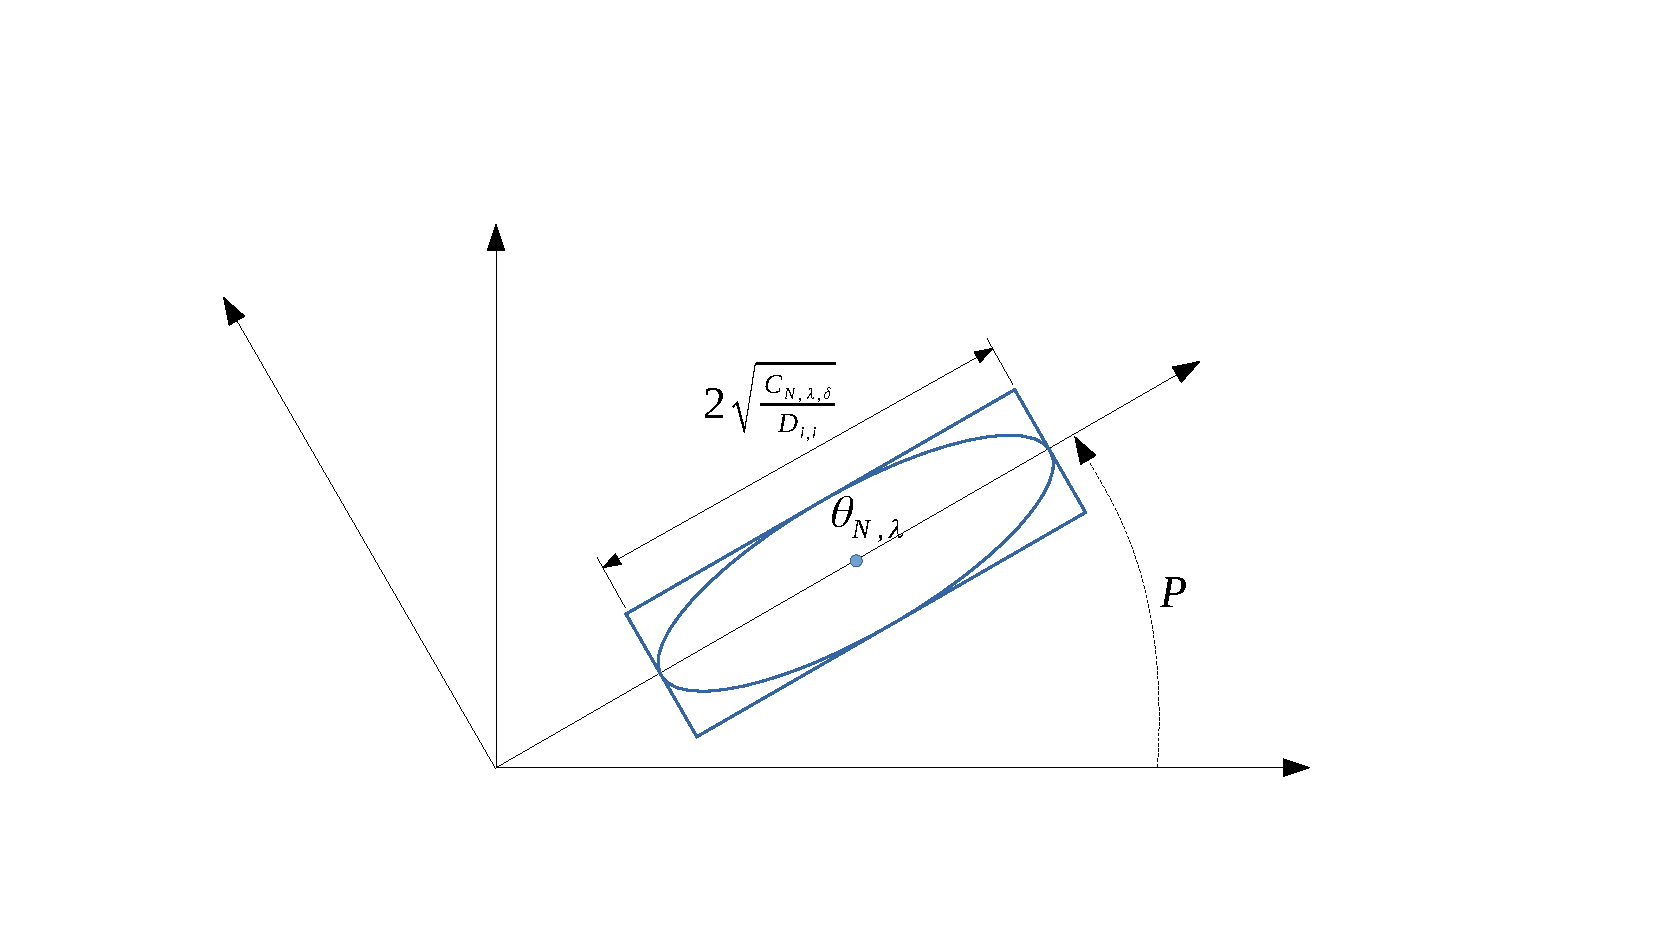
\includegraphics[trim={3.8cm, 2cm, 5cm, 3.8cm}, clip, width=0.7\linewidth]{img/ellipsoid_to_polytope}
	\caption{From the confidence ellipsoid $\cC_\delta$ to its enclosing polytope $\cP_\delta$}
	\label{fig:ellipsoid_to_polytope}
\end{figure}

\section{On the ordering of min and max}
	\label{sec:min-max-order}

	In the definition of $B_{a}^{r}(k)$ \eqref{eq:br} and $U_{a}^{r}(k)$ \eqref{eq:ur} it is essential that the minimum over the models is only taken at the end of trajectories, in the same way as for the robust objective \eqref{eq:robust-objective-discrete} in which the worst-case dynamics is only determined after the action sequence has been fully specified. Assume that $U_{a}^{r}(k)$ is instead naively defined as:
	
	\[
	U_{a}^{r}(k)=\min_{m\in[1,M]}U_{a}^{m}(k),
	\]
	
	This would not recover the robust policy, as we show in \autoref{fig:min-max-order} with a simple counter-example.
	\begin{figure}[htp]
		\centering
		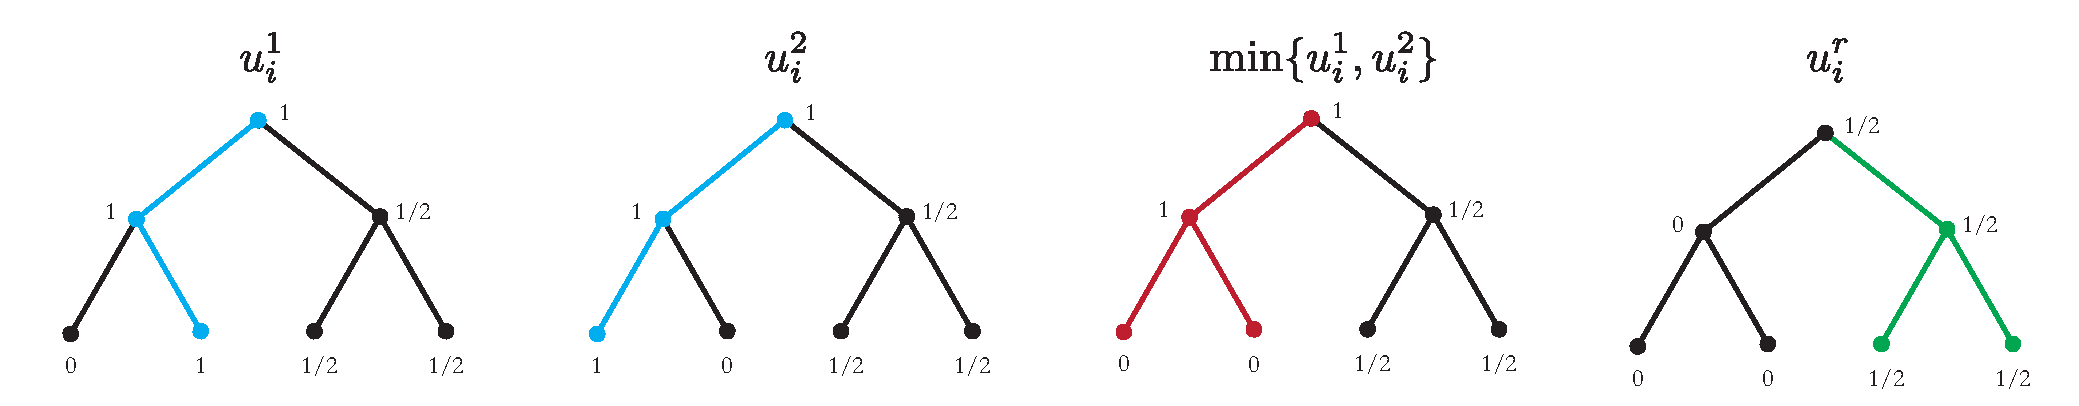
\includegraphics[width=\linewidth]{img/min-max-order}
		\caption{From left to right: two simple models and corresponding u-values with optimal sequences in blue; the naive version of the robust values returns sub-optimal paths in red; our robust U-value properly recovers the robust policy in green.}
		\label{fig:min-max-order}
	\end{figure}

\section{Experimental setting}
\label{sec:experimental-setting}

In both experiments, we used $\gamma=0.9$,  $\delta=0.9$ and a planning budget $K=100$. The perturbations were sampled uniformly in $[-0.1, 0.1]^r$ while the measurements are gaussian with covariance $\Sigma_r = 0.1 I_s$. 

\subsection{Autonomous Driving}

In the following, we describe the structure of the dynamical system $f$ representing the couplings and interactions between several vehicles.

\paragraph{Kinematics}

The kinematics of any vehicle $i\in[V]$ are represented by the Kinematic Bicycle Model:
\begin{align}
	\dot{x}_i &= v_i\cos(\psi_i), \nonumber\\
	\dot{y}_i &= v_i\sin(\psi_i), \nonumber\\
	\dot{v}_i &= a_i, \nonumber\\
	\dot{\psi}_i &= \frac{v_i}{l}tan(\beta_i), \nonumber
\end{align}
where $(x_i, y_i)$ is the vehicle position, $v_i$ is its forward velocity and $\psi_i$ is its heading, $l$ is the vehicle half-length, $a_i$ is the acceleration command and $\beta_i$ is the slip angle at the centre of gravity, used as a steering command.

\paragraph{Longitudinal control}
Longitudinal behaviour is modelled by a linear controller using three features: a desired velocity, a braking term to drive slower than the front vehicle, and a braking term to respect a safe distance to the front vehicle.

Denoting $f_i$ the index of the front vehicle preceding vehicle $i$, the acceleration command can be presented as follows:
\begin{equation*}
	a_i = \begin{bmatrix}
	\theta_{i,1} & \theta_{i,2} & \theta_{i,3}
	\end{bmatrix} \begin{bmatrix}
		v_0 - v_i \\
		-(v_{f_i}-v_i)^- \\
		-(x_{f_i} - x_i - (d_0 + v_iT))^- \\
	\end{bmatrix},
	\label{eq:theta_a}
\end{equation*}
where $v_0, d_0$ and $T$ respectively denote the speed limit, jam distance and time gap given by traffic rules.

\paragraph{Lateral control}

The lane $L_i$ with the lateral position $y_{L_i}$ and heading $\psi_{L_i}$ is tracked by a cascade controller of lateral position and heading $\beta_i$, which is selected in a way the closed-loop dynamics take the form:

\begin{align}
	\label{eq:heading-command}
    \dot{\psi}_i &= \theta_{i,5}\left(\psi_{L_i}+\sin^{-1}\left(\frac{\tilde{v}_{i,y}}{v_i}\right)-\psi_i\right),\\
    \tilde{v}_{i,y} &= \theta_{i,4} (y_{L_i}-y_i). \nonumber
\end{align}
We assume that the drivers choose their steering command $\beta_i$ such that \eqref{eq:heading-command} is always achieved: $\beta_i = \tan^{-1}(\frac{l}{v_i}\dot{\psi}_i)$.

\paragraph{LPV formulation}

The system presented so far is non-linear and must be cast into the LPV form. We approximate the non-linearities induced by the trigonometric operators through equilibrium linearisation around $y_i=y_{L_i}$ and $\psi_i=\psi_{L_i}$.

This yields the following longitudinal dynamics:
\begin{align*}
\dot{x}_i &= v_i,\\
\dot v_i &= \theta_{i,1} (v_0 - v_i) + \theta_{i,2} (v_{f_i} - v_i) + \theta_{i,3}(x_{f_i} - x_i - d_0 - v_i T),
\end{align*}
where $\theta_{i,2}$ and $\theta_{i,3}$ are set to $0$ whenever the corresponding features are not active.

It can be rewritten in the form $$\dot{X} = A(\theta)(X-X_c) + \omega.$$ For example, in the case of two vehicles only:
\begin{equation*}
    X = \begin{bmatrix}
x_i \\
x_{f_i} \\
v_i \\
v_{f_i} \\
\end{bmatrix}
,\quad
X_c = \begin{bmatrix}
-d_0-v_0 T \\
0 \\
v_0\\
v_0 \\
\end{bmatrix}
,\quad
\omega = \begin{bmatrix}
v_0 \\
v_0 \\
0\\
0\\
\end{bmatrix}
\end{equation*}

\begin{equation*}
A(\theta)
=
\begin{blockarray}{ccccc}
 & i & f_i & i & f_i \\
\begin{block}{c[cccc]}
i & 0 & 0 & 1 & 0 \\
f_i & 0 & 0 & 0 & 1 \\
i & -\theta_{i,3} & \theta_{i,3} & -\theta_{i,1}-\theta_{i,2}-\theta_{i,3} & \theta_{i,2} \\
f_i & 0 & 0 & 0 & -\theta_{f_i,1} \\
\end{block}
\end{blockarray}
\end{equation*}

The lateral dynamics are in a similar form:
\begin{equation*}
\begin{bmatrix}
\dot{y}_i \\
\dot{\psi}_i \\
\end{bmatrix}
=
\begin{bmatrix}
0 & v_i \\
-\frac{\theta_{i,4} \theta_{i,5}}{v_i} & -\theta_{i,5}
\end{bmatrix}
\begin{bmatrix}
y_i - y_{L_i} \\
\psi_i - \psi_{L_i}
\end{bmatrix}
+
\begin{bmatrix}
v_i\psi_{L_i} \\
0
\end{bmatrix}
\end{equation*}
Here, the dependency in $v_i$ is seen as an uncertain parametric dependency, \emph{i.e.} $\theta_{i,6}=v_i$, with constant bounds assumed for $v_i$ using an overset of the longitudinal interval predictor.


\paragraph{Change of coordinates}
In both cases, the obtained polytope centre $A_0$ is non-Metzler.
We use the similarity transformation of coordinates of \citet{Efimov2013}. Precisely, we choose $\Theta$ such that for any $\theta\in\Theta$, $A(\theta)$ is always diagonalisable with real eigenvalues, and perform an eigendecomposition to compute its change of basis matrix $Z$. The transformed system $X'=Z^{-1}(X-X_c)$ verifies \eqref{eq:confidence} with $A_0$ Metlzer as required to apply the interval predictor of \autoref{prop:predictor}. Finally, the obtained predictor is transformed back to the original coordinates $Z$ by using the following lemma:
\begin{lemma}[Interval arithmetic of \citealt{Efimov2012}]
	 \label{lem:interval} Let $x\in\mathbb{R}^{n}$ be a vector variable, $\underline{x}\le x\le\overline{x}$ for some $\underline{x},\overline{x}\in\mathbb{R}^{n}$. 
	
	\begin{enumerate}
		\item If $A\in\Real^{m\times n}$ is a constant matrix, then
		\begin{equation}
		A^{+}\underline{x}-A^{-}\overline{x}\le Ax\le A^{+}\overline{x}-A^{-}\underline{x}.\label{eq:Interval1}
		\end{equation}
		\item If $A\in\Real^{m\times n}$ is a matrix variable and \textup{$\underline{A}\le A\le\overline{A}$} for some $\underline{A},\overline{A}\in\Real^{m\times n}$, then
		\begin{gather}
		\underline{A}^{+}\underline{x}^{+}-\overline{A}^{+}\underline{x}^{-}-\underline{A}^{-}\overline{x}^{+}+\overline{A}^{-}\overline{x}^{-}\leq Ax\label{eq:Interval2}\\
		\leq\overline{A}^{+}\overline{x}^{+}-\underline{A}^{+}\overline{x}^{-}-\overline{A}^{-}\underline{x}^{+}+\underline{A}^{-}\underline{x}^{-}.\nonumber 
		\end{gather}
	\end{enumerate}
\end{lemma}

\paragraph{Actions}

The action space $\cA$ is constituted of five actions: faster, slower, lane change to the right, lane change to the left, and no-op. They are implemented by a lateral linear controller that track a reference lateral position $y_L$, affected by the lane change actions, and a lateral longitudinal linear controller that tracks the desired velocity $v_0$, affected by the faster and slower actions.

\paragraph{Reward}

The reward function $R$ is the following:
\[
R(x) = 
\begin{cases}
1 & \text{if the ego-vehicle is at full velocity;}\\
0 & \text{if the ego-vehicle has collided with another vehicle;}\\
0.5 & \text{else.}
\end{cases}\]

\end{document}
